\documentclass[a4paper,12pt]{book}

\usepackage[utf8x]{inputenc}
\usepackage[slovene,english]{babel}
\usepackage[pdftex]{graphicx}
\usepackage{fancyhdr}
\usepackage{amssymb}
\usepackage{amsmath}
\usepackage{algpseudocode}
\usepackage{graphicx}
\usepackage{subcaption}
\usepackage{pdfpages}
\usepackage{float}
%\usepackage{hyperxmp}
\usepackage[pdftex, colorlinks=true,
						citecolor=black, filecolor=black, 
						linkcolor=black, urlcolor=black,
						pagebackref=false, 
						pdfproducer={LaTeX}, pdfcreator={LaTeX}, hidelinks]{hyperref}

%%%%%%%%%%%%%%%%%%%%%%%%%%%%%%%%%%%%%%%%
%	DIPLOMA INFO
%%%%%%%%%%%%%%%%%%%%%%%%%%%%%%%%%%%%%%%%
\newcommand{\ttitle}{Paralelizacija evolucijskega algoritma za razporejanje opravil s kompleksnimi omejitvami}
\newcommand{\ttitleEn}{Parellelization of an evolutionary algorithm for scheduling with complex constraints}
\newcommand{\tsubject}{\ttitle}
\newcommand{\tsubjectEn}{\ttitleEn}
\newcommand{\tauthor}{Sašo Stanovnik}
\newcommand{\tkeywords}{evolucijski algoritem, paralelizacija, MPI, urnik}
\newcommand{\tkeywordsEn}{evolutionary algorithm, parallelization, MPI, timetable}
\newcommand{\temail}{sstanovnik@gmail.com}



\usepackage{hyperref}
%%%%%%%%%%%%%%%%%%%%%%%%%%%%%%%%%%%%%%%%
%	HYPERREF SETUP
%%%%%%%%%%%%%%%%%%%%%%%%%%%%%%%%%%%%%%%%
\hypersetup{pdftitle={\ttitle}}
\hypersetup{pdfsubject=\ttitleEn}
\hypersetup{pdfauthor={\tauthor, \temail}}
\hypersetup{pdfkeywords=\tkeywordsEn}


 


%%%%%%%%%%%%%%%%%%%%%%%%%%%%%%%%%%%%%%%%
% postavitev strani
%%%%%%%%%%%%%%%%%%%%%%%%%%%%%%%%%%%%%%%%  

\addtolength{\marginparwidth}{-20pt} % robovi za tisk
\addtolength{\oddsidemargin}{40pt}
\addtolength{\evensidemargin}{-40pt}

\renewcommand{\baselinestretch}{1.3} % ustrezen razmik med vrsticami
\setlength{\headheight}{15pt}        % potreben prostor na vrhu
\renewcommand{\chaptermark}[1]%
{\markboth{\MakeUppercase{\thechapter.\ #1}}{}} \renewcommand{\sectionmark}[1]%
{\markright{\MakeUppercase{\thesection.\ #1}}} \renewcommand{\headrulewidth}{0.5pt} \renewcommand{\footrulewidth}{0pt}
\fancyhf{}
\fancyhead[LE,RO]{\sl \thepage} \fancyhead[LO]{\sl \rightmark} \fancyhead[RE]{\sl \leftmark}



\newcommand{\BibTeX}{{\sc Bib}\TeX}

%%%%%%%%%%%%%%%%%%%%%%%%%%%%%%%%%%%%%%%%
% naslovi
%%%%%%%%%%%%%%%%%%%%%%%%%%%%%%%%%%%%%%%%  


\newcommand{\autfont}{\Large}
\newcommand{\titfont}{\LARGE\bf}
\newcommand{\clearemptydoublepage}{\newpage{\pagestyle{empty}\cleardoublepage}}
\setcounter{tocdepth}{1}	      % globina kazala

%%%%%%%%%%%%%%%%%%%%%%%%%%%%%%%%%%%%%%%%
% konstrukti
%%%%%%%%%%%%%%%%%%%%%%%%%%%%%%%%%%%%%%%%  
\newtheorem{izrek}{Izrek}[chapter]
\newtheorem{trditev}{Trditev}[izrek]
\newenvironment{dokaz}{\emph{Dokaz.}\ }{\hspace{\fill}{$\Box$}}

%%%%%%%%%%%%%%%%%%%%%%%%%%%%%%%%%%%%%%%%%%%%%%%%%%%%%%%%%%%%%%%%%%%%%%%%%%%%%%%
%% PDF-A
%%%%%%%%%%%%%%%%%%%%%%%%%%%%%%%%%%%%%%%%%%%%%%%%%%%%%%%%%%%%%%%%%%%%%%%%%%%%%%%

%%%%%%%%%%%%%%%%%%%%%%%%%%%%%%%%%%%%%%%% 
% define medatata
%%%%%%%%%%%%%%%%%%%%%%%%%%%%%%%%%%%%%%%% 
\def\Title{\ttitle}
\def\Author{\tauthor, \temail}
\def\Subject{\ttitleEn}
\def\Keywords{\tkeywordsEn}

%%%%%%%%%%%%%%%%%%%%%%%%%%%%%%%%%%%%%%%% 
% \convertDate converts D:20080419103507+02'00' to 2008-04-19T10:35:07+02:00
%%%%%%%%%%%%%%%%%%%%%%%%%%%%%%%%%%%%%%%% 
\def\convertDate{%
    \getYear
}

{\catcode`\D=12
 \gdef\getYear D:#1#2#3#4{\edef\xYear{#1#2#3#4}\getMonth}
}
\def\getMonth#1#2{\edef\xMonth{#1#2}\getDay}
\def\getDay#1#2{\edef\xDay{#1#2}\getHour}
\def\getHour#1#2{\edef\xHour{#1#2}\getMin}
\def\getMin#1#2{\edef\xMin{#1#2}\getSec}
\def\getSec#1#2{\edef\xSec{#1#2}\getTZh}
\def\getTZh +#1#2{\edef\xTZh{#1#2}\getTZm}
\def\getTZm '#1#2'{%
    \edef\xTZm{#1#2}%
    \edef\convDate{\xYear-\xMonth-\xDay T\xHour:\xMin:\xSec+\xTZh:\xTZm}%
}

\expandafter\convertDate\pdfcreationdate 

%%%%%%%%%%%%%%%%%%%%%%%%%%%%%%%%%%%%%%%%
% get pdftex version string
%%%%%%%%%%%%%%%%%%%%%%%%%%%%%%%%%%%%%%%% 
\newcount\countA
\countA=\pdftexversion
\advance \countA by -100
\def\pdftexVersionStr{pdfTeX-1.\the\countA.\pdftexrevision}


%%%%%%%%%%%%%%%%%%%%%%%%%%%%%%%%%%%%%%%%
% XMP data
%%%%%%%%%%%%%%%%%%%%%%%%%%%%%%%%%%%%%%%%  
\usepackage{xmpincl}
\includexmp{pdfa-1b}

%%%%%%%%%%%%%%%%%%%%%%%%%%%%%%%%%%%%%%%%
% pdfInfo
%%%%%%%%%%%%%%%%%%%%%%%%%%%%%%%%%%%%%%%%  
\pdfinfo{%
    /Title    (\ttitle)
    /Author   (\tauthor, \temail)
    /Subject  (\ttitleEn)
    /Keywords (\tkeywordsEn)
    /ModDate  (\pdfcreationdate)
    /Trapped  /False
}


%%%%%%%%%%%%%%%%%%%%%%%%%%%%%%%%%%%%%%%%%%%%%%%%%%%%%%%%%%%%%%%%%%%%%%%%%%%%%%%
%%%%%%%%%%%%%%%%%%%%%%%%%%%%%%%%%%%%%%%%%%%%%%%%%%%%%%%%%%%%%%%%%%%%%%%%%%%%%%%

\begin{document}
\selectlanguage{slovene}
\frontmatter
\setcounter{page}{1} %
\renewcommand{\thepage}{}

%%%%%%%%%%%%%%%%%%%%%%%%%%%%%%%%%%%%%%%%
%naslovnica
 \thispagestyle{empty}%
   \begin{center}
    {\large\sc Univerza v Ljubljani\\%
      Fakulteta za računalništvo in informatiko}%
    \vskip 10em%
    {\autfont \tauthor\par}%
    {\titfont \ttitle \par}%
    {\vskip 2em \textsc{DIPLOMSKO DELO\\[2mm]
    UNIVERZITETNI ŠTUDIJSKI PROGRAM PRVE STOPNJE RAČUNALNIŠTVO IN INFORMATIKA}\par}%
    \vfill\null%
    {\large \textsc{Mentor}: izr.\ prof.\ dr.  Uroš Lotrič\par}%
    {\vskip 2em \large Ljubljana 2015 \par}%
\end{center}
% prazna stran
\clearemptydoublepage

%%%%%%%%%%%%%%%%%%%%%%%%%%%%%%%%%%%%%%%%
%copyright stran
\includepdf[pages={1}]{licensepage/license.pdf}


% prazna stran
\clearemptydoublepage

%%%%%%%%%%%%%%%%%%%%%%%%%%%%%%%%%%%%%%%%
% stran 3 med uvodnimi listi
\thispagestyle{empty}
\vspace*{4cm}

\noindent
Fakulteta za računalništvo in informatiko izdaja naslednjo nalogo:
\medskip
\begin{tabbing}
\hspace{32mm}\= \hspace{6cm} \= \kill




Tematika naloge:
\end{tabbing}
Izdelajte evolucijski algoritem za razporejanje opravil, ki bo omogočal kar se da splošno vnašanje zahtev in omejitev. Algoritem preskusite na problemu sestavljanja kompleksnega urnika. Časovno potraten algoritem paralelizirajte s primerno tehnologijo. Analizirajte rezultate in uspešnost samega algoritma in njegove paralelizacije.
\vspace{15mm}






\vspace{2cm}

% prazna stran
\clearemptydoublepage

%%%%%%%%%%%%%%%%%%%%%%%%%%%%%%%%%%%%%%%%
% izjava o avtorstvu
\vspace*{1cm}
\begin{center}
{\Large \textbf{\sc Izjava o avtorstvu diplomskega dela}}
\end{center}

\vspace{1cm}
\noindent Spodaj podpisani \tauthor\ sem avtor  diplomskega dela z naslovom:

\vspace{0.5cm}
\emph{\ttitle}

\vspace{1.5cm}
\noindent S svojim podpisom zagotavljam, da:
\begin{itemize}
	\item sem diplomsko delo izdelal samostojno pod mentorstvom
		izr.\ prof.\ dr.\ Uroša Lotriča,

	\item	so elektronska oblika diplomskega dela, naslov (slov., angl.), povzetek (slov., angl.) ter ključne besede (slov., angl.) identični s tiskano obliko diplomskega dela,
	\item soglašam z javno objavo elektronske oblike diplomskega dela na svetovnem spletu preko univerzitetnega spletnega arhiva.	
\end{itemize}

\vspace{1cm}
\noindent V Ljubljani, dne 10. 9. 2015 \hfill Podpis avtorja:

% prazna stran
\clearemptydoublepage



\includepdf[pages={1}]{nipponpage/nippon.pdf}




% prazna stran
\clearemptydoublepage

%%%%%%%%%%%%%%%%%%%%%%%%%%%%%%%%%%%%%%%%
% kazalo
\def\thepage{}% preprecimo tezave s stevilkami strani v kazalu
\tableofcontents{}


% prazna stran
\clearemptydoublepage

%%%%%%%%%%%%%%%%%%%%%%%%%%%%%%%%%%%%%%%%
% povzetek
\addcontentsline{toc}{chapter}{Povzetek}
\chapter*{Povzetek}
V delu se osredotočimo na problem generiranja urnikov s paraleliziranim evolucijskim algoritmom. Raziščemo pogosto uporabljene metode razporejanja opravil ter ugotovimo, katere so primerne za primere s kompleksnimi omejitvami in izberemo paralelizacijsko shemo, ki je najbolj ustrezna za učinkovit izračun. Prav tako izberemo primerno predstavitev podatkov, ki se sklada z genetskimi operatorji in kriterijsko funkcijo, ki lahko enostavno pokrije velik nabor kompleksnih omejitev. Implementiramo in paraleliziramo razširljiv algoritem za izračun rešitev ter raziščemo uspešnost generiranja. Predstavimo način minimizacije prostorske kompleksnosti problema s pametnim deljenjem dela med procesi. Lastnosti paralelnega programa analiziramo skozi podrobno analizo časov izvajanja in teoretično analizo paralelizacije. 
\bigskip

\noindent\textbf{Ključne besede:} \tkeywords.
% prazna stran
\clearemptydoublepage

%%%%%%%%%%%%%%%%%%%%%%%%%%%%%%%%%%%%%%%%
% abstract
\selectlanguage{english}
\addcontentsline{toc}{chapter}{Abstract}
\chapter*{Abstract}
The focus of our work is on the problem of generating a timetable using a parallel evolutionary algorithm. We explore commonly used scheduling methods and determine their suitability for cases with complex constraints, then select a parallelization scheme most suitable for efficient computation. Furthermore, we choose a data representation that best complements genetic operators and the fitness function, which covers a wide range of complex constraints. We implement and parallelize an extensible algorithm for computing solutions to our problem. A method of minimizing the space complexity of the problem by efficiently dividing data between processes is also described. We analyse the properties of our solution through a thorough analysis of run times and memory consumptions coupled with a theoretical analysis of the results. 
\bigskip

\noindent\textbf{Keywords:} \tkeywordsEn.
\selectlanguage{slovene}
% prazna stran
\clearemptydoublepage

%%%%%%%%%%%%%%%%%%%%%%%%%%%%%%%%%%%%%%%%
\mainmatter
\setcounter{page}{1}
\pagestyle{fancy}


\chapter{Uvod}
Razvrščanje opravil je širok pojem, ki zajema teme, kot so organiziranje lastnega časa, razvrščanje procesov v industrijski proizvodnji ter ustvarjanje optimalnih urnikov. Veliko strokovne pozornosti je požel predvsem slednji problem, saj se v praksi pogosto pojavlja ter zanj ne obstaja ena sama rešitev, ki bi ustrezala vsem. Zanima nas, kakšne rešitve na področju generiranja urnikov že obstajajo, kakšni pristopi so pogosto uporabljeni, da lahko pretehtamo prednosti in slabosti ter implementiramo svojo rešitev, ki ustreza praktičnim kriterijem. Vse to želimo implementirati s paralelno shemo, ki bo pohitrila izvajanje programa in omogočala, da rešimo večji problem, kot bi ga lahko sicer sekvenčno. 


\section{Cilj}
V sklopu diplomske naloge smo se osredotočali na učinkovito reševanje problema generiranja urnika v velikem problemskem prostoru z mnogimi atributi in omejitvami. Poskušali smo najti učinkovito predstavitev problemskega prostora, ki ustreza izbrani paralelizacijski shemi, in v kriterijsko funkcijo vključiti čimveč omejitev in preprek iz realne problemske domene. Stremeli smo k implementaciji, ki ni poenostavljena ter se čim bolj približa zahtevam, ki jih postavlja domena v realnem življenju. 

Velik cilj implementacije je bila enostavnost in učinkovitost dodajanja novih kriterijev razvrščanja, saj se kaže, da je generiranje urnikov velikokrat težavno zaradi raznovrstnih in kompleksnih omejitev, ki jih postavijo posamezniki. Te omejitve so lahko čisto očitne narave ali pa so samo implicitne, ki se jih posamezniki ne zavedajo, a jih vseeno občutijo. Če je sistem za omejitve dovolj razumljiv in preprost za spremembe, potem jih lahko implementiramo več, a morda za ceno učinkovitosti. 

Ker je problemski prostor realnih urnikov zelo velik ter rešitev (dobrih in slabih) nepredstavljivo mnogo, je potrebno poskrbeti za hitro izvajanje izračuna. V današnjem svetu ne primanjkuje procesorskih kapacitet, zato se ni potrebno osredotočati izključno na učinkovitost, tako kot v preteklosti, ko so bili računalniki veliko manj zmogljivi. Lahko izkoristimo dejstvo, da imajo že računalniki, ki jih imamo doma, več jeder, in zaradi tega lahko učinkovito izvajajo več hkratnih izračunov. Paralelizacija iskanja čim boljše rešitve je učinkovit način za pohitritev izračunov, ki so v našem primeru zelo primerni za vzporeden izračun.

Da bi uporabili izkušnje mnogih raziskovalcev pred nami, smo morali pregledati že uporabljene pristope, predstavitve podatkov ter paralelizacijske sheme, ki so bile uporabljene za reševanje takih in podobnih problemov. Ugotovili smo, kateri pristopi so primerni za naš cilj in kako bi lahko izboljšali posamezne dele teh, da sestavimo čim bolj učinkovito rešitev. 

Rešitev smo preiskusili najprej na podatkih, ki smo jih generirali sami, potem pa še na resničnih podatkih za generiranje urnika Fakultete za računalni\-štvo in informatiko Univerze v Ljubljani. 


\section{Pregled področja}
Leta 1962 je Gotlieb raziskoval in predstavil \cite{gotlieb1962construction} prvotno različico {problema}, ki je za današnje pojme poenostavljena, a je vseeno povedla raziskovalce v mnogo raziskav o lastnostih problema. Kmalu so se začele pojavljati raziskave same rešljivosti \cite{neufeld1974graph}, ki so analizirale, ali je teoretično možno sestaviti tak urnik, da bo zadoščal enostavnim kriterijem prekrivanj. Za predstavitev so bili uporabljeni grafi, na podlagi katerih so določali rešljivost. 

Čez čas so se raziskave usmerile v kompleksnost rešitve \cite{cooper1996complexity,even1975complexity}. Zaradi same velikosti problemskega prostora je kmalu postalo jasno, da iskanje točno najboljše rešitve ni izvedljivo. Če točne rešitve ne moremo najti, je potrebno najti čim boljši približek, čemur služijo hevristične metode preiskovanja prostora. Posebej popularne metode so postale metode evolucijskih algoritmov, kot sta simulacija kaljenja ter genetski algoritmi \cite{sigl2003solving,wall1996genetic,burke1998simple,abdullah2008generating,colorni1992genetic}.

Evolucijski algoritmi sami po sebi niso popolna metoda za iskanje rešitev problema. Uporabimo jih lahko za učinkovito preiskovanje problemskega prostora, a so lahko dokaj časovno neučinkoviti, če mamo velik problem ali pa hočemo zelo dober približek najboljše rešitve. Z vzponom superračunalnikov ter zmogljivih strojev, ki jih imamo na voljo, so se raziskave usmerile v pohitritve izvajanja algoritmov s paralelizacijo. Zaradi same narave genetskih algoritmov---možno jih je namreč enostavno paralelizirati---je nastalo veliko rešitev za vzporeden izračun \cite{alba2002parallelism, abramson1991parallel}. Uporabljene so bile drevesne strukture na enotnih in ločenih sistemih ter različne strategije večnivojskega izračuna. 

Raziskovalci so uporabljali različne predstavitve podatkov problema, kot sta večdimenzionalna predstavitev fiksne velikosti, podobna kvadru \cite{sigl2003solving}, ter matrična predstavitev \cite{colorni1992genetic}. Avtorji se zavedajo, da je predstavitev zelo pomembna za učinkovito iskanje, saj je potrebno konsistentno izvajati operatorje križanja in mutacije nad posameznikom. Potrebno je tudi paziti, da izberemo predstavitev, ki nam pomaga izločiti popolnoma nemogoče rešitve hitro in učinkovito. 

Tudi danes problem še ni definitivno rešen, saj se še vedno pojavlja veliko člankov, ki poskuša rešiti problem na nove načine ali pa izboljšati stare \cite{dun2014simulated,ansari2015comparing}. Za generiranje urnikov obstaja veliko orodij, ki omogočajo različne nivoje prilagodljivosti ter uporabljajo različne načine izračunov. Pojavila so se podjetja, ki se ukvarjajo izključno z rešitvami za ustvarjenje urnikov, saj je to področje široko in obstaja redna potreba po celem svetu. Ker so te komercialne rešitve zaprte in plačljive narave, jih nismo analizirali. 



\chapter{Problemska domena}

\section{Razvrščanje opravil}
Razvrščanje opravil je v praksi zelo pogost in izjemno težek problem --- od leta 1975 je več raziskovalcev dokazalo, da je NP-poln \cite{even1975complexity,cooper1996complexity,sigl2003solving}. Podane imamo pogoje za veljavnost rešitve --- urnika --- in pa pogoje, ki nam povedo, katera rešitev je boljša od druge. V splošnem obstajajo sredstva, ki se časovno v rešitvi ne smejo prekrivati, sredstva, ki se lahko, omejitve uporabe sredstev, mehke zahteve glede razporeditve in tako dalje. V sistemu urnikov izobraževalne ustanove je precej več omejitev, implicitnih ali eksplicitnih, kot je sprva razvidno. V implementaciji smo se osredotočili na omejitve, ki so smiselne in občutno zvišajo kakovost urnika. 

Potrebno se je tudi zavedati, da je kakovost urnika težko izmeriti in, v nekaterih primerih, tudi težko definirati. V vsakem parametru kvalitete lahko zlahka določimo boljše in slabše rešitve: manj prekrivanj je očitno boljše, enakomerne obremenitve so boljše od neenakomernih. Težava nastane, ko je potrebno ovrednotiti kombinacije teh parametrov. Potrebno se je odločiti, kateri kriteriji so bolj pomembni od drugih ter jim pripisati vrednost na merljivi skali. Kot bomo videli, je temu izjemno primerna kriterijska funkcija evolucijskih algoritmov, ki temelji prav na definiranih kriterijih za kakovost posameznika in na podlagi teh izbira najboljše. 

Če primerjamo urnike z drugimi področji razvrščanja opravil, lahko takoj opazimo, da pri urnikih zaporedje vnosov v veliki večini, razen če to ni definirano s specifičnim kriterijem, ni pomembno. To nam poenostavi izračun, saj nam ni potrebno preverjati vnaprej določenega zaporedja vnosov. 

\subsection{Omejitve}
\label{sec:fitness-items}
Ker iščemo rešitev čim večje kakovosti, moramo postaviti kriterije za to kakovost. Uvedli bomo trde in mehke omejitve: trde omejitve so tiste, ki preprečujejo veljavnost rešitve in se jim je potrebno popolnoma izogniti, da je rešitev sploh uporabna. Mehke omejitve so v resnici sestavljene iz dveh logičnih delov. Prvi so vzorci, ki, če so prisotni, slabšajo kvaliteto rešitve, drugi pa jo izboljšujejo. 

V kriterijski funkciji vse sklope obravnavamo podobno: pripišemo jim številsko vrednost. Trde omejitve imajo visoko negativno vrednost. Mehke omejitve, ki izboljšujejo rešitev, imajo relativno manjšo pozitivno vrednost, tiste, ki rešitev slabšajo, pa imajo relativno manjšo negativno vrednost. Iz tega sledi, da je boljša rešitev tista, ki je bolj pozitivna. 
\\
\\
Naštejmo najprej trde, ki smo jih upoštevali v implementaciji:
\begin{itemize}
\item Prostor ne sme biti zaseden več kot enkrat ob istem času.
\item Vaje morajo biti v dvojnih ciklih.
\item Izvajalec ne sme imeti dveh vnosov ob istem času. 
\item Termini pred 7:00 ali po 20:00 niso dovoljeni. 
\item Predavanja in vaje istega predmeta se ne smejo časovno prekrivati. 
\item Predavanja istega predmeta se ne smejo časovno prekrivati.
\item Asistenti ne smejo imeti obremenitve nad določeno mejo. 
\item Prostora ne sme zasedati več študentov, kot to prostor dovoljuje. 
\end{itemize}

\vspace{5ex}
\noindent Mehke omejitve:
\begin{itemize}
\item Študentu naj se vnosi ne bi prekrivali. 
\item Vnosi naj ne bodo pred določeno ali po določeni uri.
\item Predavanja naj bodo združena. 
\item Študenti naj imajo vnose razporejene kompaktno. 
\item Predavanja naj bodo pred vsemi vajami v istem tednu. 
\end{itemize}

\noindent
Nekaj komentarjev glede zgornjih omejitev: študentom je omogočeno prekrivanje vnosov, saj se drugače lahko zgodi, da problem ni rešljiv. Z variacijo uteži, ki jo podamo temu kriteriju, lahko določimo, kako močno se trudimo izboljšati rešitve s takimi lastnostmi. Pravila mehke narave prispevajo k rešitvi takrat, ko je ta že ``uporabna'': zaradi velike razlike v uteži med trdimi in mehkimi omejitvami na začetku izračuna prevladuje iskanje posameznikov, ki ustrezajo čim manj trdim omejitvam, šele nato, ko se število uveljavljenih trdih omejitev ustali, pa se začne poznati učinek mehkih omejitev. Slednje potrebujemo zato, da v nadaljevanju izračuna izboljšamo sicer možno rešitev ter da ne izberemo samo naključne, ki sicer ustreza najstrožjim kriterijem, je pa v resnici lahko slaba. 

\subsection{Problemski prostor}
Število možnih rešitev za določen problem je lahko izjemno veliko. Vse kombinacije študentov, predmetov, prostorov, dni in ur tudi v manjših problemih doprinesejo do neobvladljivega števila rešitev. Lokalnih ekstremov je veliko, zato moramo poskrbeti, da se v njih ne zataknemo. 

Z večanjem števila trdih omejitev lahko izjemno hitro omejimo število možnih rešitev, z mehkimi omejitvami pa spreminjamo poti, po katerih bomo iskali boljše rešitve. Določeno skrb je potrebno posvetiti temu, da imamo v implementaciji dovolj dober generator naključnih števil, da lahko nepristransko raziščemo čim več problemskega prostora. 


\section{Evolucijski algoritmi}
Evolucijski algoritmi so način hevrističnega preiskovanja prostora, ki so navdihnjeni z naravno evolucijo. Uporabljajo operatorje, kot so mutacija, križa\-nje in selekcija, da ustvarjajo nove generacije populacije tako, da ohranjajo dobre lastnosti posameznikov in kombinirajo lastnosti prednikov. Znana poddružina algoritmov so genetski algoritmi. V splošnem imajo evolucijski algoritmi naslednje 4 stopnje:  

\begin{enumerate}
\item Generiraj začetno populacijo. 
\item Dokler ne dosežemo ustavitvenega pogoja, ponavljaj naslednja koraka. 
\item Iz populacije izberi preživele s pomočjo kriterijske funkcije.
\item Iz preživelih generiraj novo generacijo populacije z operatorji, kot sta križanje in mutacija. 
\end{enumerate}

Na koncu iz celotne populacije izberemo najboljšega posameznika glede na vrednost kriterijske funkcije. Evolucijski algoritmi nimajo točno določenega ustavitvenega kriterija, izbrati si ga moramo sami. Pogosti izbiri sta čas in dosežena določena vrednost kriterijske funkcije, lahko pa ga prekinemo tudi ročno ali takrat, ko se rešitev neha izboljševati skozi generacije. 

Optimizacijski problemi so v praksi velikokrat \cite{cooper1996complexity} preveč kompleksni, da bi bilo iskanje točne oziroma najboljše rešitve praktično ali celo izvedljivo. Za reševanje se uporabljajo hevristične metode preiskovanja prostora, kot je sekvenčna metoda, ki so jo avtorji uporabili v \cite{burke1998simple}. Zelo razširjen je razred evolucijskih algoritmov, ki simulirajo razvoj živih bitij skozi emulacijo postopka evolucije. Glavni cilj teh algoritmov je iskanje približka optimalne rešitve skozi kombinacije posameznikov skozi mnogo generacij. Znan je razred genetskih algoritmov, ki so podskupina evolucijskih, in postavljajo omejitve na predstavitev podatkov in metode genetskih operatorjev: predstavitev naj bi bila fiksne dolžine, genetski operatorji pa tam delujejo nad posameznimi odseki genov na način, ki izkorišča fiksno dolžino in poravnanost predstavitve. 

Nadvse pomemben del njih je kriterijska funkcija, s katero ocenimo ustreznost rešitve --- posameznika v naši domeni. Z njo določimo, kateri posamezniki iz posamezne generacije populacije preživijo in ustvarijo potomce za naslednjo generacijo. Pomembno se je zavedati, da je ta ocena le približek in je morda pristranska glede na tistega, ki je dodeljeval uteži različnim kriterijem. 

Pri izbiri preživelih obstaja veliko načinov odločanja \cite{thierens1994convergence}. Lahko preprosto izberemo $n$ najboljših, ali pa se spustimo v simulacijo dejanske selekcije. Selekcija z ruleto (ang. \emph{roulette-wheel selection}) izbere posameznike z verjetnostjo, ki je sorazmerna z njihovo oceno ustreznosti. Rangirna selekcija (ang. \emph{ranking selection}) priredi ta postopek tako, da lahko posameznikom na podlagi vrednosti kriterijske funkcije priredi drugačno verjetnost preživetja. Kot zelo učinkovit in prilagodljiv način izbora preživelih se v praksi izkaže \cite{miller1995genetic} turnirska selekcija, ki ustvari tekmovanja med posamezniki: vsakič, ko je potrebno izbrati novega preživelega, naključno izberemo $k$ posameznikov, izmed njih pa preživi tisti, ki ima najboljšo ustreznost. Učinkovit je tudi za kriterijske funkcije, ki imajo veliko šuma \cite{miller1995genetic} zaradi ``nepopolnosti''. 

Za to, da ne zapademo v lokalne ekstreme pri iskanju rešitve, je pomembno tudi, da ne obdržimo samo najboljših rešitev. Slabše rešitve imajo lahko dele, ki so boljši od delov, ki jih imajo boljše rešitve. Ti deli se lahko s križanjem kombinirajo v skupno boljšega posameznika. Turnirska selekcija omogoča preživetje slabših posameznikov, saj je izbor skupin naključen. 

Pogosti parametri evolucijskih algoritmov so: velikost populacije v nekaj tisoč posameznikih, velika verjetnost križanja in majhna verjetnost mutacije (to se sklada z resničnimi geni) ter razmeroma elitističen pristop do selekcije. Evolucijske algoritme lahko implementiramo samo s križanjem, kar presenetljivo ne kaže slabih rezultatov, a je mutacija pomembna za fine spremembe v posameznikih, hitrejšo pridobitev rešitve in reševanje iz lokalnih ekstremov. Elitističen pristop pa tudi pospešuje hitrost iskanja, saj hitreje favoriziramo najboljše. To ne pomeni, da vedno izberemo le najboljše (čeprav se lahko odločimo, da najboljših $n$ vedno preživi), pomeni le, da naj svojo metodo selekcije izberemo tako, da bodo boljši posamezniki imeli večjo možnost preživetja. Število oziroma razmerje preživelih naj ne bi bilo preveliko, saj hočemo, da se nova populacija generira iz izbrane skupine preživelih in ne iz velikega dela prejšnje generacije, saj bi to pomenilo, da je v izvirni populaciji manjši delež dobrih posameznikov. 



\section{Vzporedno računanje}
Če želimo program paralelizirati, je potrebno imeti več enot, ki lahko izvajajo program ali njegove dele, vzporedno. V osnovi so to večprocesorski sistemi, ki so danes prisotni v večini računalnikov. Lahko uporabimo dodatno strojno opremo, kot so grafične kartice, ki lahko zelo hitro izvajajo specifične tipe programov, ali pa uporabimo namensko strojno premo za izračun, kot je Intel Xeon Phi. Če želimo uporabiti kapacitete več sistemov naenkrat, jih lahko povežemo v večračunalniški sistem. Bolj dostopne so rešitve, kjer povežemo več ločenih sistemov preko komunikacijskega kanala (za kar lahko uporabimo MPI), lahko pa uporabimo sisteme z uniformnim pomnilnikom. 

\subsection{Izbira paralelizacijske sheme}
Pri izbiri paralelizacijske sheme določenega programa je potrebno upoštevati njegove lastnosti. Paralelizacija na grafičnih karticah deluje najbolje, ko so podatki neodvisni in je problem možno razdeliti na več delov ter se vsi deli izvajajo sočasno (brez različnih vejitev). Koprocesorji, kot so Intel Xeon Phi \cite{xeonphi}, dobro delujejo pri izračunih, za katere lahko uporabimo vektorsko enoto, še posebej ukaz FMA (\emph{Fused Multiply--Add}). Obe omenjeni tehnologiji tudi potrebujeta določeno strojno opremo, kar lahko močno omeji število sistemov, na katerih je možno pognati program.

Standard MPI (\emph{Message Passing Interface}) omogoča povezavo posameznih jeder procesorja v enem sistemu ali pa med oddaljenimi računalniki. Temelji na izmenjavi sporočil med posameznimi procesi, ki med seboj niso nujno identični. Vsakemu procesu je pripisan identifikator (\textit{rang}), ki pooseblja proces pri pošiljanju sporočil. Implementacija MPI v ozadju skrbi za čim bolj učinkovito izmenjavo sporočil in podpira veliko vzorcev pošiljanja: komunikacijo točka-točka, oddajanje, zbiranje, raztros in krčenje. Prav tako se implementacije zavedajo lokalnosti (ali nelokalnosti) jeder in za pošiljanje med njimi uporabijo najboljšo pot: naj bo to deljen pomnilnik \cite{mpisharedmemory} ali pa sklad TCP/IP. 

Preučili smo možnost kombiniranja MPI in OpenMP. Slednji služi enostavni in učinkoviti paralelizaciji znotraj enega sistema s pomočjo učinkovite komunikacije med nitmi preko deljenega pomnilnika ter zaklepanjem, ki ga ponuja sistemska implementacija. Naša motivacija je bila, da bi komunikacijo in paralelizacijo znotraj vsakega sistema izvedli preko OpenMP, komunikacijo med različnimi procesi pa preko povezav, ki bi jih ustvarili z MPI. Spoznali smo \cite{hybridmpiopenmp}, da hibridna implementacija med MPI in OpenMP v praksi ne deluje tako dobro, kot bi pričakovali, saj prihaja do nižanja zmogljivosti zaradi več režijskega dela zaradi hkratne uporabe dveh paralelizacijskih shem, prednosti komunikacije z deljenim pomnilnikom pa tudi ne bi imeli, saj MPI samodejno zazna osnovno topologijo in za komunikacijo na enem sistemu lahko uporablja deljeni pomnilnik (odvisno od implementacije standarda). Večjo težavo predstavlja težavno programiranje. Lahko imamo težave z režijo komunikacije: odločiti se moramo, ali naj prekrivamo komunikacijo in izračune, da bomo učinkoviti, ali naj počakamo, da vse niti zaključijo, nato pa samo glavna nit pošlje podatke. Vse to moramo tudi pravilno implementirati. Poleg tega so tudi razlike v implementacijah knjižnic MPI (npr. OpenMPI, MPICH), ki ne zagotavljajo vedno varnosti niti ali pa ne nudijo ogrodja za večnitno programiranje, ki ga ponuja standard MPI. 

Jezika C in Fortran sta podprta neposredno v samem standardu MPI, jeziku naše implementacije (C++) pa so dostopne le funkcionalnosti iz implementacije za jezik C, kar ne omogoča preprostega pošiljanja vsebovalnikov, ki jih ponuja C++, kot je \texttt{std::vector}. V ta namen smo uporabili knjižnico Boost \cite{boost}, ki ovija funkcionalnosti implementacije MPI s podpornimi funkcijami, ki olajšajo delo s standardnimi vzorci programiranje v C++. Uporabili smo komponenti \texttt{Boost.MPI} in \texttt{Boost.Serialization}: prva ponuja ovojnico prek funkcionalnosti MPI, druga pa omogoča definiranje in kompaktno shranjevanje struktur, ki jih določimo kot uporabniki. Te strukture se potem pošiljajo preko vmesnikov MPI, Boost.Serialization pa poskrbi, da se kazalci na vse strukture pravilno vzpostavijo. 

V standardu MPI točen način komunikacije med procesi ni definiran, a je prepuščen posamezni implementaciji. V osnovi se računalniki povežejo brez posebnega orodja in le izvajajo program s toliko procesi, kolikor jih dodelimo. Uporabimo lahko tudi upravljalnik poslov, kjer centralni računalnik nadzira poljubno mnogo drugih računalnikov in na njih poganja opravila, ki jih podamo. Ti so bolj napredni programi in lahko pametno delijo procese med sisteme, zadržijo procese v vrsti ter avtomatsko shranjujejo status in izhode. 



\chapter{Implementacija}
Paraleliziran algoritem smo implementirali v jeziku C++ s pomočjo knjižnic Boost in MPI. Uporabili smo Python skripte za generiranje podatkov ter kontroliran zaporedni zagon velikega števila programov, nato pa z njimi zajeli izhod ter ga analizirali in obdelali. Ker smo za potrebe poganjanja programa na različnih sistemih morali vzpostaviti primerno okolje z vso potrebno opremo, smo ustvarili Bash skripto, ki samodejno pridobi, prevede in namesti vse potrebne komponente ter nastavi okoljske spremenljivke na sveži namestitvi operacijskega sistema Ubuntu 15.04. Za prikaz rezultatov smo izvozili rezultat v format JSON in podatke prikazali v spletni aplikaciji, za katero smo uporabili HTML, JavaScript in CSS. 


\section{Vhodni podatki}
Za vhodne podatke smo oblikovali sheme XML (\emph{Extensible Markup Language}) v obliki dokumentov XSD (\emph{XML Schema Definition}). Vhodni podatki so tako vnešeni v obliki dokumentov XML, kar omogoča lažje branje, spreminjanje in ustvarjanje podatkov. Prav tako nam je pravilnost vhodnih podatkov v veliki meri zagotovljena s skladnostjo s shemo. 

Vsak tip vhodnega podatka (študent, učilnica, učitelj in predmet) je definiran v svoji datoteki --- seveda več osebkov v eni. Prav tako v ločeni datoteki določimo splošne nastavitve za evolucijski algoritem. 

Ustvarili smo program za generiranje vhodnih podatkov na osnovi števila študentov, učilnic, predmetov in drugih splošnih značilnosti. Ti podatki so grob približek realnih, so pa uporabni za preizkušanje različnih velikosti problema. 


\section{Evolucijski algoritem}
Genetski algoritem smo implementirali modularno in v skladu z načeli dobrega kodiranja. Poskrbeli smo za učinkovito izrabo pomnilnika, za učinkovit izračun kriterijske funkcije na posameznikih populacije pa smo uporabili dodatne podatkovne strukture, ki so nekoliko zvišale porabo pomnilnika, a so zmanjšale časovno zahtevnost. Vsak vnos v urniku smo predstavili z enim objektom, a smo omejili vnose na enourne. To pomeni, da so npr. predavanja, ki trajajo tri zaporedne ure, sestavljena iz treh ločenih vnosov. 

V domeni evolucijskih algoritmov je zelo pomembna predstavitev posameznika. Genetski algoritmi predpostavljajo, da je zapis linearen in fiksne dolžine, kar za predstavitev posameznega urnika ni primerno. Razlog tiči v tem, da  ni nujno, da dve rešitvi zavzemata enako količino prostora zaradi porazdelitev študentov po učilnicah. Prav tako je težko določiti smiselno ureditev podatkov, saj urnik nima popolne naravne ureditve. Možna je ureditev po času, a po tem obstaja dilema, kateri kriterij uporabiti za nadaljnje razvrščanje enakovrednih vnosov. 

Skozi raziskave predstavitev podatkov v obstoječih študijah \cite{sigl2003solving,abramson1991parallel,colorni1992genetic} smo se odločili za zelo fleksibilno predstavitev, ki omogoča enostaven izračun kriterijske funkcije, saj je to najbolj časovno potraten in kompleksen del algoritma. Poleg tega si želimo, da je generiranje posameznikov nove generacije možno enostavno implementirati na način, ki ne daje nesmiselnih rezultatov. Vsak urnik predstavimo z (neurejenim) zaporedjem vnosov, ki so logično razvidni v urniku. Prednost tega pristopa pred večdimenzionalnimi tabelami vrednosti kot v \cite{sigl2003solving}, je to, da ne porabljamo prostora po nepotrebnem. 
\\
\\
Vsak vnos vsebuje identifikator(je): 
\begin{itemize}
\item učilnic, 
\item učiteljev, 
\item predmetov, 
\item terminov, 
\item študentov, ki so vezani na vnos,
\item ter vrednosti, ki označujejo, ali je to vnos predavanj ali vaj.
\end{itemize}

\noindent
Ta predstavitev, poleg omogočanja učinkovitih izračunov, ponuja tudi visoko prostorsko učinkovitost, saj ne shranjujemo nepotrebnega praznega prostora kot v primeru večdimenzionalne matrike vrednosti. 


\subsection{Križanje}
V sklopu evolucijskih algoritmov izstopajo genetski algoritmi, ki imajo značil\-ne karakteristike križanja, še posebej v povezavi s tem, da je zapis posameznika fiksne dolžine. Obstaja enotočkovno križanje, kjer se linearen zapis sestavi iz dveh delov, vsak iz svojega prednika. V $n$-točkovnem križanju je takih delov več, v uniformnem križanju pa za vsak znak v nasledniku naključno izberemo prednika. 

Take strategije križanja niso primerne za naš zapis posameznikov, saj ti nimajo stroge ureditve ter niso fiksne dolžine. Odločili smo se za način podoben uniformnemu križanju, saj slednji kaže dobre rezultate \cite{spears1995virtues}. Kot znak obravnavamo posamezen predmet in nato kombiniramo različne lastnosti: 

\begin{enumerate}
\item Kombiniramo celotne predmete. 
\item Izberemo le razporeditev skupin študentov iz enega predmeta in vse ostale lastnosti iz drugega. 
\item Izberemo razporeditev učiteljev iz enega, vse ostale lastnosti iz drugega. 
\item Izberemo učilnice enega ter vse ostale lastnosti drugega. 
\end{enumerate}

Strategijo seveda vsakič izberemo naključno, a je enaka za celotnega posameznika. Če v kakšni od strategij 2--4 opazimo, da se število vnosov obeh predmetov ne sklada, naključno izberemo enega od obeh predmetov ter ga prepišemo v rezultat nespremenjenega. To naredimo zato, ker ne obstaja smiselna bijektivna funkcija iz enega v drugega, ki bi ohranila integriteto posameznika. 

Vsi načini križanja ohranjajo smiselnost rešitve, torej ne ustvarjajo napak, ki jih je enostavno preprečiti. Na primer nikoli ne podvajajo študentov v vnosih, ne ustvarjajo neobstoječih vrednosti in ohranjajo strukturo podatkov. Za samo veljavnost rešitve tukaj ne skrbimo, saj za to obstaja kriterijska funkcija, ki penalizira nemogoče posameznike. 

\subsection{Mutacija}
Mutacijo lahko vzamemo kot najbolj trivialen del evolucijskega algoritma, saj je potrebno samo naključno spremeniti eno vrednost. Zaradi omejitev domene se izkaže, da je spreminjanje samo ene vrednosti bolj kompleksno, kot je opazno na prvi pogled. Kot pri križanju imamo tudi tukaj paleto strategij. Če je preživeli posameznik izbran za mutacijo, se na enem vnosu izvrši naključno izbrana strategija izmed naslednjih: 

\begin{enumerate}
\item \label{mutation:1} Vnosu spremenimo učilnico. 
\item \label{mutation:2} Vnosu spremenimo dan. 
\item \label{mutation:3} Vnosu spremenimo uro.
\item \label{mutation:4} Vnosu spremenimo dan in uro. 
\item \label{mutation:5} Kombiniramo in premešamo študente dveh vnosov vaj pri istem predmetu. 
\item \label{mutation:6} Vnosu spremenimo učitelja. 
\end{enumerate}

Pri vseh možnostih je potrebno biti pozoren na priključene vnose. To so predavanja istega predmeta, ki so časovno ena zraven drugih ter dvojni cikli vaj, ki vsebujejo iste študente. Pri možnosti \ref{mutation:1} spremenimo učilnico vsem priključenim vnosom, ne glede na to, ali so to predavanja ali vaje. Za možnosti \ref{mutation:2}, \ref{mutation:3} in \ref{mutation:4} spremenimo samo priključene vaje, saj so te nujno v dvournih terminih, predavanja je pa možno razbiti na več delov. Ker je za rešitev urnika zelo pomembna časovna razporeditev vnosov, imamo tukaj tri možnosti za časovno mutacijo namesto le ene. Možnost \ref{mutation:5} uporabimo samo pri vajah (predavanj ne spreminjamo) in seveda upoštevamo vnose, enako velja tudi za možnost \ref{mutation:6}. 

\subsection{Kriterijska funkcija}
S pazljivo implementacijo mutacij in križanj si lahko izjemno pomagamo pri hitrosti in enostavnosti implementacije kriterijske funkcije. Znebimo se lahko mnogih preverjanj integritete in pravilnosti rešitve, če vemo, da smo generirali brez določenih napak in teh napak nismo ustvarjali z mutacijami in križanji. Te napake vključujejo stvari, kot so to, da ustvarimo študenta, ki ne obstaja, študentu dodamo predmet, ki ga nima oziroma sploh ne obstaja, in podobno. 

V naši implementaciji lahko kriterijska funkcija zavzame vsa števila. Višja (bolj pozitivna) števila pomenijo boljšega posameznika. Trde omejitve smo implementirali z zelo visoko negativno vrednostjo, mehke omejitve pa z manjšo negativno ali pozitivno, odvisno od potrebe pogoja. 

Implementirali smo vse omejitve, omenjene v poglavju \ref{sec:fitness-items}. S smiselno uporabo kompromisov prostora za čas smo dosegli algoritemsko kompleksnost $O(n^2)$, kjer je $n$ število vnosov v posamezniku populacije. Vsak par vnosov smo primerjali le enkrat. Za vsako točko iz omejitev smo šteli ponovitve, nato pa rezultatu prišteli zmnožek števila ponovitev in uteži, ki smo jo pripisali določeni pojavitvi. Negativne uteži so pomenile slabši rezultat. 

Večina omejitev je za implementacijo trivialna, netrivialna pa je omejitev, ki vrednoti kompaktnost predavanj. To smo implementirali kot normalizirano razliko med varianco časovne razporeditve vnosov enakomerne porazdelitve ter porazdelitve, ki jo ima določen posameznik. Ta omejitev je tako delovala na dnevni ravni, kjer je združevala vnose znotraj enega dneva, kot tudi na tedenski ravni, ko je združevala vnose po celotnem tednu in si prizadevala, da bi bil kakšen dan lahko prost. 


\subsection{Selekcija}
Za način selekcije smo implementirali turnirsko selekcijo. Tekmovanja smo organizirali tako, da smo naključno premešali posameznike v populaciji in jo nato razdelili na toliko delov, kolikor preživelih smo potrebovali. Poskusili smo dva načina izbire zmagovalca vsakega tekmovanja: v prvem načinu smo izbrali tistega, katerega indeks je vrnila eksponentna porazdelitev z določenim parametrom, v drugem načinu pa smo preprosto izbrali najboljšega. Empirični preizkusi so pokazali, da algoritem hitreje konvergira z drugim načinom, zato smo ga uporabili kot končno rešitev. 

Vredno je omeniti, da s tem načinom selekcije vedno preživi najboljši posameznik v populaciji, saj zmaga v katerikoli skupini, v katero je izbran. To vnese določeno mero elitizma in poskrbi, da imamo manjšo verjetnost, da kakovost populacije začne padati. 

\section{Paralelizacija}
Za paralelizacijo smo si izbrali MPI in temu primerno prilagodili paralelizacijsko shemo. Procesi so si med seboj v večini enakovredni. Posebno vlogo ima le glavni proces (proces $0$), ki opravlja nekaj dodatnih nalog. Na začetku iz svojega okolja pobere nastavitve in vhodne podatke, jih obdela in rezultate razpošlje vsem. Med samim algoritmom je zadolžen za selekcijo, a le za izvajanje tekmovanj --- izračun kriterijske funkcije se dogaja porazdeljeno na procesih, iz katerih posamezniki izhajajo. Na koncu se v sistemu glavnega procesa generira končni rezultat programa. 

\let\oldfigurename\figurename
\renewcommand{\figurename}{Algoritem}
\begin{figure}
\caption{Potek glavnega dela programa. }
\label{alg:main}
\begin{algorithmic}[1]
\Function{program}{}
	\If{glavni proces}
		\State preberi vhodne podatke;
		\State razpošlji nastavitve in vhodne podatke; \label{alg:main:initialsend}
	\EndIf
	\State generiraj začetno populacijo;
	\For{generacija}
		\State izračunaj kriterijsko funkcijo na vsakem posamezniku;
		\State pošlji vrednosti glavnemu procesu; \label{alg:main:fitnessgather}
		\If{glavni proces}
			\State izvedi selekcijo;
			\State razpošlji identifikatorje preživelih; \label{alg:main:survivorindicesbroadcast}
		\EndIf
		\State filtriraj populacijo v preživele;
		\State razpošlji preživele vsem ostalim; \label{alg:main:survivorbroadcast}
		\State prerazporedi populacijo glede na zmogljivosti procesov; \label{alg:main:adjustment}
		\State izvedi repopulacijo;
	\EndFor
	\State najdi najboljšega posameznika v vsakem delu populacije;
	\State pošlji najboljšega posameznika glavnemu procesu; \label{alg:main:bestbroadcast}
	\If{glavni proces}
		\State najdi najboljšega posameznika;
		\State izpiši rezultat na podlagi najboljšega;
	\EndIf
\EndFunction
\end{algorithmic}
\end{figure}
\let\figurename\oldfigurename

Algoritem poteka glavnega programa s poudarjenimi deli komunikacije in paralelizacije vidimo v algoritmu \ref{alg:main}. Pošiljanje se izvaja v vrsticah \ref{alg:main:initialsend}, \ref{alg:main:fitnessgather}, \ref{alg:main:survivorindicesbroadcast}, \ref{alg:main:survivorbroadcast}, \ref{alg:main:adjustment} in \ref{alg:main:bestbroadcast}. V vrstici \ref{alg:main:adjustment} pošiljanje ni eksplicitno napisano, a za potrebe prerazporeditve vsi procesi pošljejo čas izvajanja glavnemu procesu, ki nato prerazporedi populacijo med procese in to razpošlje nazaj. Diagram \ref{img:diagram} služi lažji predstavitvi poteka programa ter razporeditvi dela in pošiljanja med procesi. 

\begin{figure}
\makebox[\textwidth]{\includegraphics[scale=0.55]{res/diagram.pdf}}
\caption{Diagram poteka programa. }
\label{img:diagram}
\end{figure}

Za učinkovitost in porabo časa za pošiljanje so pomembne vrstice \ref{alg:main:fitnessgather}, \ref{alg:main:survivorindicesbroadcast}, \ref{alg:main:survivorbroadcast} in \ref{alg:main:adjustment}. Od vseh je najbolj zahtevno pošiljanje celotnih preživelih v načinu vsi-vsem (\texttt{MPI\_Allgather}) v vrstici \ref{alg:main:survivorbroadcast}, saj je tukaj, poleg latence, ki je enaka pri vseh pojavitvah komunikacije, prisotna tudi razmeroma velika količina podatkov, saj pošiljamo kompleksne strukture vnosov v urniku. Ker smo previdno implementirali podatkovno strukturo za vnos v urniku, je slednja velika le $4 + 2s + p$ bajtov, kjer je $s$ število študentov v vnosu in $p$ število procesov v vnosu. V preiskusnem naboru podatkov z 250 študenti, 20 predmeti in 20 učitelji je tako velikost enega posameznika približno 8 kB. V populaciji velikosti 5000 posameznikov, razmerjem preživelih $0{,}01$ in s 4 procesi tako vsak proces pošlje 100 kB podatkov. Ta količina ni velika za pošiljanje v enem sistemu, a lahko predstavlja veliko oviro, če povezava med ločenimi sistemi ni dobra ali pa je počasna. 

V naši implementaciji se populacija izmenja v vsaki generaciji. To je dobro za iskanje rešitve, saj s tem povečamo raznolikost zaloge posameznikov, ki jo ima vsak proces na voljo za sestavljanje naslednje generacije. Tako lahko hitreje preiščemo prostor in se ne zadržujemo v območju, ki bi ga umetno ustvarili, če bi imeli lokalne populacije, ki bi se vsakih $n$ generacij izmenjale med procesi. 


\subsection{Računska in prostorska zahtevnost}
Poleg minimiziranja velikosti struktur za zmanjšanje časa, potrebnega za pošiljanje, smo tudi smiselno omejili podatke, ki se pošiljajo. Celotna populacija nikoli ne obstaja na enem samem procesu (razen v primeru enega samega procesa). Vsak proces generira le en del populacije, nato pa okoli razpošlje le preživele, ki jih je izbral glavni proces. To pomeni, da se prepošilja občutno manjši del podatkov in močno pripomore k hitrosti delovanja programa. 

Čas izračuna in pošiljanja ni edina skrb pri paralelizaciji programov. Prostorska kompleksnost je lahko velika skrb v sistemih z velikim številom procesov, saj se lahko poraba pomnilnika močno poveča s tem, ko se poveča število procesov. S porazdelitvijo celotne populacije učinkovito porazdelimo porabo pomnilnika. 

Prav tako se program samodejno prilagaja zmogljivostim sistemov, na katerih teče. Naša rešitev podrobno meri čas izvajanja različnih delov izračuna in nato prilagodi število posameznikov, ki jih ima posamezen proces tako, da so vsi procesi zasedeni čim več časa. S premikajočim povprečjem izravna ekstremne vrednosti in tako dopušča nekaj časa ostalim programom, ki tečejo v ozadju. Na ta način se izognemo nepotrebnemu čakanju na počasnejše sisteme, ki sodelujejo v izračunu. 



\chapter{Rezultati}
Program smo poganjali na različnih kombinacijah naslednjih sistemov:
\begin{enumerate}
\item 8-jedrni Intel\textsuperscript\textregistered\ i7 3770K @ 4.3 GHz, 8 GB RAM na virtualnem stroju Ubuntu 15.04, gostovan na Windows 10 z VMware Workstation, \label{computer:virtual}
\item 2-jedrni Intel\textsuperscript\textregistered\ Core 2 Duo E8500 @ 3.5 GHz, 4GB R AM na Ubuntu Server 15.04, \label{computer:old}
\item 4-jedrni Intel\textsuperscript\textregistered\ Core i5-4278U @ 2.6 GHz, 8 GB RAM na OS X 10.10. \label{computer:laptop}
\end{enumerate}

Na sistemih \ref{computer:virtual} in \ref{computer:old} smo uporabljali prevajalnik Clang 3.6.0, na sistemu \ref{computer:laptop} pa Apple LLVM 6.1.0 (Clang-602.0.63), ki je enakovreden verziji 3.6.0. Za prevajanje smo uporabili naslednjo skupino zastavic: \texttt{-std=c++11 -Wall -Wextra -pedantic -pipe -Wno-unused-parameter -O3 -march=native}. Za upravljanje smo uporabili sistem CMake. 

\section{Simulirani vhodni podatki}
Za potrebe kontroliranega testiranja s podatki zmernih velikosti smo en testni nabor avtomatsko zgenerirali s pomočjo Python skripte. Skupno število študentov v treh letnikih smo nastavili na 235. Prvima dvema letnikoma smo dodelili po 5 predmetov, tretjemu pa 10. V prvih dveh letnikih smo uporabili vse predmete kot obvezne, v tretjem samo enega. Ostale, neobvezne predmete, smo enakomerno porazdelili med študente letnika. Vsakemu predmetu smo pripisali svojega profesorja, število asistentov pa smo omejili na 10 in jim predmete enakomerno porazdelili. Število predavalnic smo omejili na 4, od katerih se lahko 2 uporabita kot učilnici za vaje. Namenske učilnice za vaje so 3. Posebnih zahtev glede učilnic nismo določili, tako so se vsi predmeti lahko izvajali v vseh učilnicah. 

Za vse primere smo pri zagonu programa uporabili razmerje preživelih (glede na celotno populacijo) $0{,}01$, verjetnost mutacije $0{,}15$ in verjetnostjo križanja $0{,}85$. Vrednosti parametrov smo dobili z empiričnim iskanjem takih, ki omogočajo hitro konvergiranje. Prav tako se ranga vrednosti skladata z vrednostmi, ki ju navaja literatura \cite{pongcharoen2002determining}. Merjenje časa smo implementirali interno, da smo lahko podrobno merili čas izvajanja posameznega dela programa. V ta namen smo uporabili časovnike iz standardne knjižnice \texttt{std::chrono}. Za merjenje porabe pomnilnika smo uporabili orodje \texttt{top} in izpisali vrednost \texttt{RES} -- pomnilnik, ki ga je alociral proces, brez deljenih knjižnic. 

\subsection{Čas izvajanja}
Zmanjšanje časa izvajanja je večinoma prvi cilj paralelizacije. Slika \ref{pic:processes-times} prikazuje čase izvajanja generacij programa s tem, ko programu dodelimo več procesov, v obliki več škatel z brki. Črta povezuje povprečja posameznih vnosov. Zadnje tri vrednosti so zaradi preglednosti prikaza pomaknjene proti levi in niso sorazmerne s skalo predhodnih vrednosti. Vse nastavitve programa, razen števila dodeljenih procesov, so bile v vseh primerih enake. Velikost populacije je bila 5000. 

Opazimo lahko, da nam je paralelizacija uspela. Čas izvajanja se hitro zmanjšuje do štirih vzporednih procesov in počasi nadaljnje zmanjšuje do osmih procesov. Od tam naprej se ustali in začne zelo počasi zviševati. Tako zmanjšanje vrednosti je popolnoma v skladu s pričakovanji. Sistem \ref{computer:virtual} ima dodeljenih 8 procesorskih jeder, a so 4 jedra navidezna zaradi tehnologije Intel\textsuperscript\textregistered\ Hyper-Threading, ki navidezno podvoji število fizičnih jeder in tako omogoči vzporednim procesom, da si delijo procesorske vire. Ta navidezna jedra seveda niso enako zmogljiva, kot bi bila fizična, a vseeno doprinesejo pohitritev zaradi izkoriščenja prej neizkoriščenih delov procesorja. 

V območju, kjer število procesov preseže število (logičnih) jeder, ne moremo pričakovati pohitritev v smiselno paraleliziranem programu. Tam ne izkoriščamo nobenih dodatnih zmogljivosti sistema, a samo povečujemo režijske stroške pošiljanja in upravljanja s procesi. Opazimo tudi, da se varianca časov manjša do osmih vzporednih procesov, potem pa se ponovno začne zviševati. To je posledica upravljalnika s procesi operacijskega sistema, ki med izvajanjem nedeterministično preklaplja med procesi. 

\begin{figure}
	\centering
	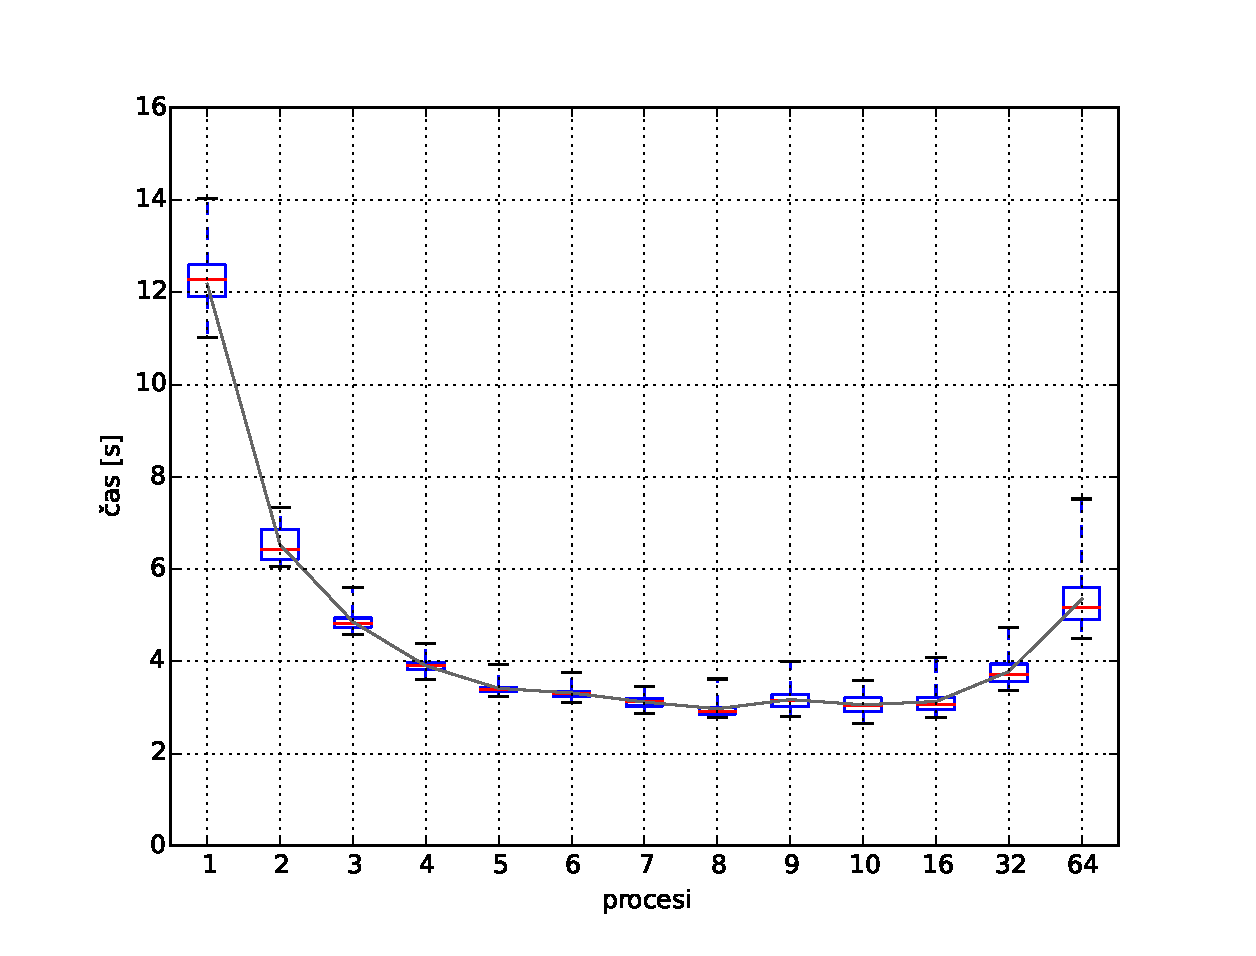
\includegraphics[scale=0.55]{res/processes-times.eps}
	\caption{Povezava med številom jeder in časom izvajanja programa na sistemu \ref{computer:virtual}. }
	\label{pic:processes-times}
\end{figure}

\subsection{Teoretična analiza časov izvajanja}
Zgoraj omenjene rezultate lahko potrdimo tudi z analizo pohitritve in učinko\-vitosti. Najprej definirajmo nekaj osnovnih oznak. $t_s(n)$ označuje čas izvajanja sekvenčnega programa pri določeni velikosti problema $n$ in $t_p(n,p)$ čas izvajanja paralelnega programa velikosti $n$ s $p$ procesi. 

Pohitritev (enačba \ref{eqn:speedup}) je mera, ki nam pove, kolikokrat hitreje se naš program izvaja glede na sekvenčno verzijo. 
\begin{equation}
\label{eqn:speedup}
S(n,p) = \frac{t_s(n)}{t_p(n,p)}
\end{equation}

Učinkovitost (enačba \ref{eqn:efficiency}) je podobna mera, ki meri, kakšen je delež izrabe procesorjev in nam pove, kolikšnega dela procesorskih moči ne izkoriščamo zaradi sekvenčnih delov programa in režijskih stroškov komunikacije. Vrednosti so v območju $0 \leq E(n,p) \leq 1$, razen v primeru superlinearnih pohitritev, ko je učinkovitost lahko večja od 1. 

\begin{equation}
\label{eqn:efficiency}
E(n,p) = \frac{S(n,p)}{p}
\end{equation}

Podatke najdemo v tabeli \ref{tab:efficiency-speedup-karp}, grafično predstavitev pa v sliki \ref{pic:speedup-efficiency}. Največja pohitritev na sistemu \ref{computer:virtual} je pri osmih vzporednih procesih, kjer je pohitritev štirikratna glede na sekvenčno izvajanje programa. Učinkovitost linearno pada zaradi režijskih stroškov komunikacije pri več procesih. Kot pričakovano največ pridobimo, ko dodamo prvi dodatni proces, nato se pohitritve napram enemu procesu manj manjšajo. Nad osmimi vzporednimi procesi dodatne pohitritve ne opazimo več, pri velikem zvečanju števila procesov (32 in 64) pa opazimo močno zmanjšanje pohitritve in učinkovitosti programa. 

\begin{figure}
	\centering
	\includegraphics[scale=0.6]{res/speedup-efficiency.eps}
	\caption{Pohitritev in učinkovitost algoritma, izmerjena na sistemu \ref{computer:virtual}}
	\label{pic:speedup-efficiency}
\end{figure}

Ugotovimo še časovne deleže izvajanja programa. S podrobnimi meritvami različnih delov programa lahko izračunamo deleže sekvenčnega izvajanja (deli programa, ki se izvajajo le na procesu 1), paralelnega izvajanja in komunikacije. Del programa izven samega izračuna generacij populacije smo izpustili, saj ti za paralelizacijo niso pomembni in so za izvajanje trivialno hitri. Izračune naredimo tako, da za vsako kategorijo meritve povprečimo čase vseh procesov, nato pa izračunamo deleže časov izvajanja. Pri enem samem procesu se seveda ves paralelni čas prišteje k sekvenčnemu. Za izračun smo uporabili rezultate iz sistema \ref{computer:virtual} z velikostjo populacije 5000. 

Tabela \ref{tab:time-ratios} prikazuje čas in deleže časa za vse tri naštete kategorije. Vidimo, da se program sekvenčno izvaja zanemarljivo malo časa, saj je edina posebna naloga glavnega procesa pri glavnem izračunu selekcija, ki je pa zelo hitra. Pri številu procesov, ki je manjše ali enako številu razpoložljivih jeder na sistemu, je delež paralelnega izvajanja med 80 in 90 \%. S povečevanjem števila jeder se poveča časovni delež komunikacije dokaj konstantno, ko pa število procesov preseže število razpoložljivih jeder, se začne paralelni delež močno nižati na račun komunikacije. Skozi povečanje velikosti populacije se deleži ne spremenijo opazno. 

S temi vrednostmi lahko izračunamo Karp-Flattovo metriko $e$ (enačba \ref{eqn:karp}, vrednosti v tabeli \ref{tab:efficiency-speedup-karp}). S pomočjo te metrike lahko preko eksperimentalnih meritev izvemo, kolikšnega deleža programa ne moremo pohitriti. Tako lahko tudi sklepamo, ali se pri povečanju števila procesov zveča tudi delež komunikacije. 

\begin{equation}
\label{eqn:karp}
e = \frac{\sigma(n) + \kappa(n,p)}{t_s(n)}
\end{equation}

Sekvenčni delež programa predstavlja $\sigma(n)$, $\kappa(n,p)$ pa čas komunikacije. Iz tabele \ref{tab:efficiency-speedup-karp} je razvidno, da matrika variira, a v okviru našega sistema ne narašča, kar pomeni, da se strošek komunikacije ne veča. Ko je število procesov nad zmogljivostjo sistema (8), metrika kot pričakovano narašča, saj se veča delež komunikacije zaradi relativno manj zmogljive arhitekture. 

\begin{table}
\centering
\caption{Podatki za pohitritev, učinkovitost in Karp-Flattovo metriko za različno število procesov. }
\label{tab:efficiency-speedup-karp}
\begin{tabular}{r | c | c | c}
$p$ & $S(n,p)$ & $E(n,p)$ & $e$ \\
\hline
1 & $1{,}000$ & $1{,}000$ & / \\
2 & $1{,}864$ & $0{,}932$ & $0{,}063$ \\
3 & $2{,}507$ & $0{,}836$ & $0{,}049$ \\
4 & $3{,}121$ & $0{,}780$ & $0{,}043$ \\
5 & $3{,}567$ & $0{,}713$ & $0{,}040$ \\
6 & $3{,}675$ & $0{,}613$ & $0{,}038$ \\
7 & $3{,}907$ & $0{,}558$ & $0{,}039$ \\
8 & $4{,}097$ & $0{,}512$ & $0{,}049$ \\
9 & $3{,}841$ & $0{,}427$ & $0{,}059$ \\
10 & $3{,}982$ & $0{,}398$ & $0{,}068$ \\
16 & $3{,}893$ & $0{,}243$ & $0{,}062$ \\
32 & $3{,}223$ & $0{,}101$ & $0{,}097$ \\
64 & $2{,}276$ & $0{,}036$ & $0{,}19$ \\
\end{tabular}
\end{table}


\begin{table}[H]
\centering
\caption{Časi izvajanja programa (in njihovi deleži) za populacijo \mbox{$N = 5000$} na sistemu \ref{computer:virtual}. }
\label{tab:time-ratios}
\begin{tabular}{r | c | c | c}
p & sekvenčni del & paralelni del & komunikacija \\
\hline
1 & 2448 s $(0{,}947)$ & / & 85 s $(0{,}033)$ \\
2 & $0{,}08$ s $(0{,}0000)$ & 1160 s $(0{,}884)$ & 153 s $(0{,}116)$ \\
3 & $0{,}08$ s $(0{,}0000)$ & 857 s $(0{,}877)$ & 119 s $(0{,}113)$ \\
4 & $0{,}09$ s $(0{,}0001)$ & 679 s $(0{,}866)$ & 105 s $(0{,}134)$ \\
5 & $0{,}10$ s $(0{,}0001)$ & 589 s $(0{,}859)$ & 97 s $(0{,}141)$ \\
6 & $0{,}11$ s $(0{,}0002)$ & 573 s $(0{,}860)$ & 93 s $(0{,}141)$ \\
7 & $0{,}12$ s $(0{,}0001)$ & 531 s $(0{,}847)$ & 95 s $(0{,}153)$ \\
8 & $0{,}13$ s $(0{,}0002)$ & 479 s $(0{,}800)$ & 119 s $(0{,}199)$ \\
9 & $0{,}12$ s $(0{,}0001)$ & 493 s $(0{,}773)$ & 144 s $(0{,}227)$ \\
10 & $0{,}10$ s $(0{,}0001)$ & 447 s $(0{,}728)$ & 167 s $(0{,}272)$ \\
16 & $0{,}11$ s $(0{,}0001)$ & 479 s $(0{,}759)$ & 152 s $(0{,}241)$ \\
32 & $0{,}12$ s $(0{,}0002)$ & 522 s $(0{,}687)$ & 238 s $(0{,}313)$ \\
64 & $0{,}25$ s $(0{,}0002)$ & 611 s $(0{,}567)$ & 467 s $(0{,}433)$ \\
\end{tabular}
\end{table}

Časi izračuna generacije variirajo v območju $0{,}2$ s, ko je povprečen čas 4 s in v območju 2 s, ko je povprečen čas 19 s. Opazili smo tudi znatno povišanje časa izračuna za do 30 \% ko smo na sistemu počeli nekaj poleg izvajanja samega programa. Sistema sicer med testiranjem nismo uporabljali, zato to ne doprinese veliko k celotnemu času. Ker je sekvenčni program v našem primeru isti kot paralelni, a izvajan na le enem procesu, imamo nekaj nepotrebnih klicev za komunikacijo. V tabeli \ref{tab:time-ratios} vidimo, da je to okoli \mbox{3 \%} celotnega časa izvajanja programa. Na podlagi teh podatkov v meritvah dovoljujemo napako 5 \%. 

\subsection{Prostorska kompleksnost}
Količina pomnilnika, ki ga program zavzame, ponavadi ni cilj paralelizacije, je pa pomembna skrb, saj lahko z neprevidno paralelizacijo in povečanjem števila procesov presežemo količino razpoložljivega pomnilnika. Poleg deljenja časa izračuna je potrebno razdeliti tudi podatke, drugače se lahko izjemno poveča prostorska kompleksnost. 

Sliki \ref{pic:processes-ram} in \ref{pic:processes-ram-normalized} prikazujeta spreminjanje porabe pomnilnika z večanjem števila jeder. Slika \ref{pic:processes-ram} prikazuje povprečno porabo enega procesa, slika \ref{pic:processes-ram-normalized} pa skupno porabo vseh procesov. Vidimo, da smo uspešno implementirali tudi porazdelitev podatkov med procese, saj poraba narašča linearno v odvisnosti od števila procesov (\ref{pic:processes-ram-normalized}). To je najboljša možna situacija, saj smo enakomerno razdelili populacijo med procese. Vredno je omeniti, da se poraba pomnilnika med procesi na istem sistemu razlikuje minimalno, je pa tudi odvisna od zmogljivosti sistema zaradi našega sistema prilagajanja razpoložljivim sredstvom. 

\begin{figure}	
	\centering
	\includegraphics[scale=0.5]{res/processes-ram.eps}
	\caption{Razmerje med številom procesov in porabo pomnilnika enega procesa. }
	\label{pic:processes-ram}
\end{figure}
\begin{figure}
	\centering
	\includegraphics[scale=0.5]{res/processes-ram-normalized.eps}
	\caption{Razmerje med številom procesov in porabo pomnilnika vseh procesov skupaj. }
	\label{pic:processes-ram-normalized}
\end{figure}

Z večanjem števila jeder lahko izboljšamo čas izvajanja in s tem pohitrimo program. Če želimo povečati problem, lahko poleg drugačnih (večjih, bolj kompleksnih) vhodnih podatkov povečamo velikost posamezne generacije. Na sliki \ref{pic:population-ram} opazimo, da se z večanjem velikosti populacije linearno veča tudi poraba pomnilnika vsakega procesa, kar pomeni, da se linearno veča tudi poraba pomnilnika celotne skupine procesov. Linearno povečanje prostorske kompleksnosti kaže, da smo uspešno razdelili populacijo in je noben proces po nepotrebnem ne podvaja. 

\begin{figure}
	\centering
	\includegraphics[scale=0.5]{res/population-ram.eps}
	\caption{Povezava med velikostjo populacije in porabo pomnilnika vsakega procesa. }
	\label{pic:population-ram}
\end{figure}


\subsection{Evolucijski algoritem}
Poglejmo si še obnašanje našega algoritma na bolj finem nivoju. Zanima nas učinkovitost našega algoritma za porazdeljevanje dela glede na zmogljivosti ter stabilnost časov izvajanja. Pri procesih, ki so povezani preko MPI, je zelo pomembna pot pošiljanja podatkov, saj hitrost in latenca močno vplivata na zmogljivost celotnega sistema. Program smo pognali na sistemih \ref{computer:virtual}, \ref{computer:old} in \ref{computer:laptop} ter jih povezali fizično, z Ethernet kabli, in brezžično preko omrežja WiFi. 

Sliki \ref{pic:generation-time-wifi} in \ref{pic:generation-time-eth} prikazujeta ta dva primera. Obakrat smo program pognali z identičnimi nastavitvami, edina razlika je bila povezava med sistemi. Povprečen čas izvajanja na sliki \ref{pic:generation-time-wifi} je 3.99 s, na sliki \ref{pic:generation-time-eth} pa je znižan na 3.08 s. Opazimo lahko tudi značilno bolj enakomerno in konstantno porazdelitev časov za vsako generacijo, ker je latenca med sistemi manjša in povezava bolj stabilna. 

V obeh primerih, še posebej na sliki \ref{pic:generation-time-eth}, je opazen učinek algoritma za prilagajanje razpoložljivim kapacitetam. Še posebej v prvih nekaj deset generacijah je ta učinek poudarjen, saj vsi procesi začnejo z enako veliko populacijo, potem se pa čez čas prilagodijo. 

\begin{figure}
	\centering
	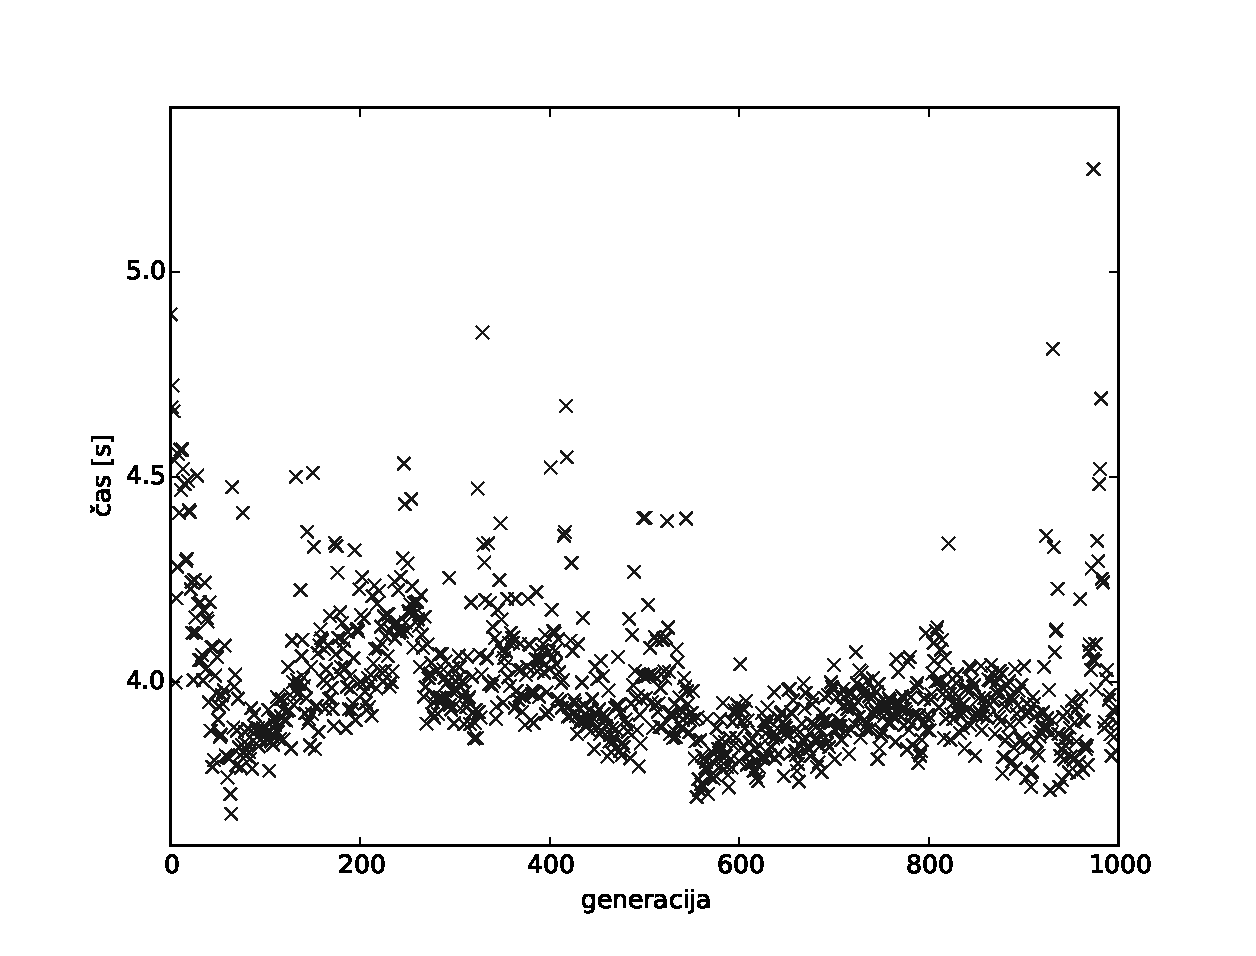
\includegraphics[scale=0.5]{res/generation-time-three-wifi.eps}
	\caption{Časi za izračun generacij na sistemih \ref{computer:virtual}, \ref{computer:old} in \ref{computer:laptop} povezanih preko omrežja WiFi. }
	\label{pic:generation-time-wifi}
\end{figure}
\begin{figure}
	\centering
	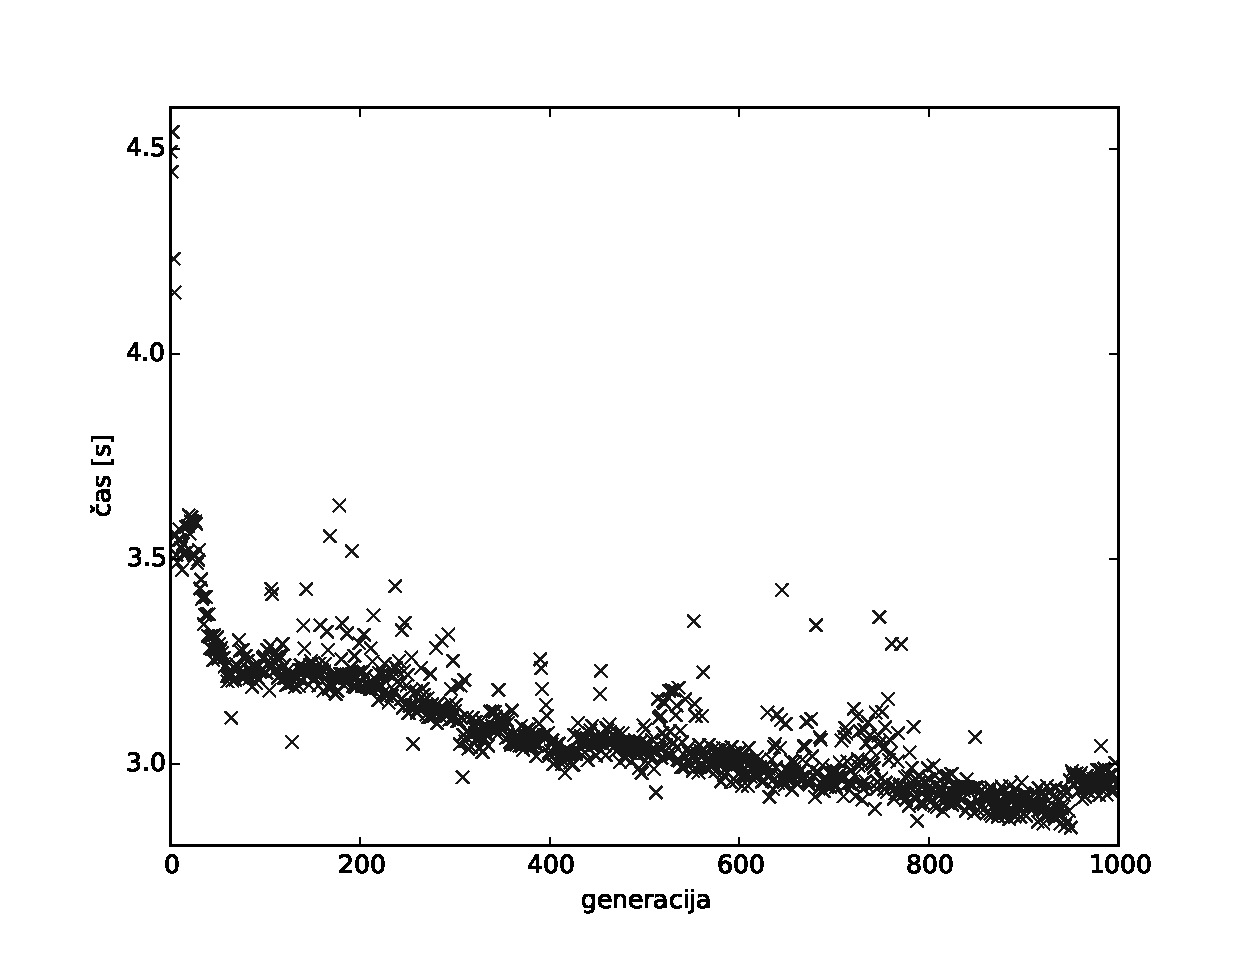
\includegraphics[scale=0.5]{res/generation-time-three-eth.eps}
	\caption{Časi za izračun generacij na sistemih \ref{computer:virtual}, \ref{computer:old} in \ref{computer:laptop} povezanih preko omrežja Ethernet. }
	\label{pic:generation-time-eth}
\end{figure}

Velikost populacije vpliva tudi na hitrost iskanja rešitve: efektivno večja populacija pomeni, da preiskujemo večji del problemskega prostora in hitreje najdemo boljšo rešitev. Slika \ref{pic:generation-fitness-multiple} prikazuje ustreznosti najboljšega posameznika v populaciji skozi generacije za tri velikosti populacije. 

Opazimo, da zvišanje velikosti populacije močno vpliva na hitrost iskanja rešitve, še posebej v začetnih generacijah. Vrednosti se v nadaljnjih generacijah ne ustalijo tako, kot prikazuje graf. Vrednosti na začetku so zelo majhne (negativne), ker imamo tako definirano kriterijsko funkcijo: preprečevalnim omejitvam pripišemo veliko negativno vrednost. Ko se pojavitve preprečevalnih omejitev izločijo, pridejo v poštev izboljševalne omejitve, ki imajo občutno manjše vrednosti. Takšna ustalitev vrednosti ne pomeni, da je algoritem končan. Dobro je, če spremljamo rezultat in se na podlagi slednjega odločimo, ali algoritem zaključimo. Dober primer so prekrivanja vaj pri študentih. Ker je prekrivanj v osnovi veliko, ima ta omejitev majhno težo. Tisoč omejitev ali sto omejitev ima lahko veliko semantično razliko, a če upoštevamo, da je razlika v ustreznosti le majhen del kazni za npr. prekrivanje predavanj profesorja, na grafu ne opazimo razlike. V naših poskusih se je pri populaciji velikosti 5000 rešitev, ki ima nič ali izjemno malo prekrivanj, pojavila okoli generacije 300. Na to seveda vplivajo uteži, ki jih podamo programu. Zaradi proste izbire pri ustavitvenem pogoju pa moramo sami ugotoviti, ali nam rešitev ustreza. 

\begin{figure}
	\centering
	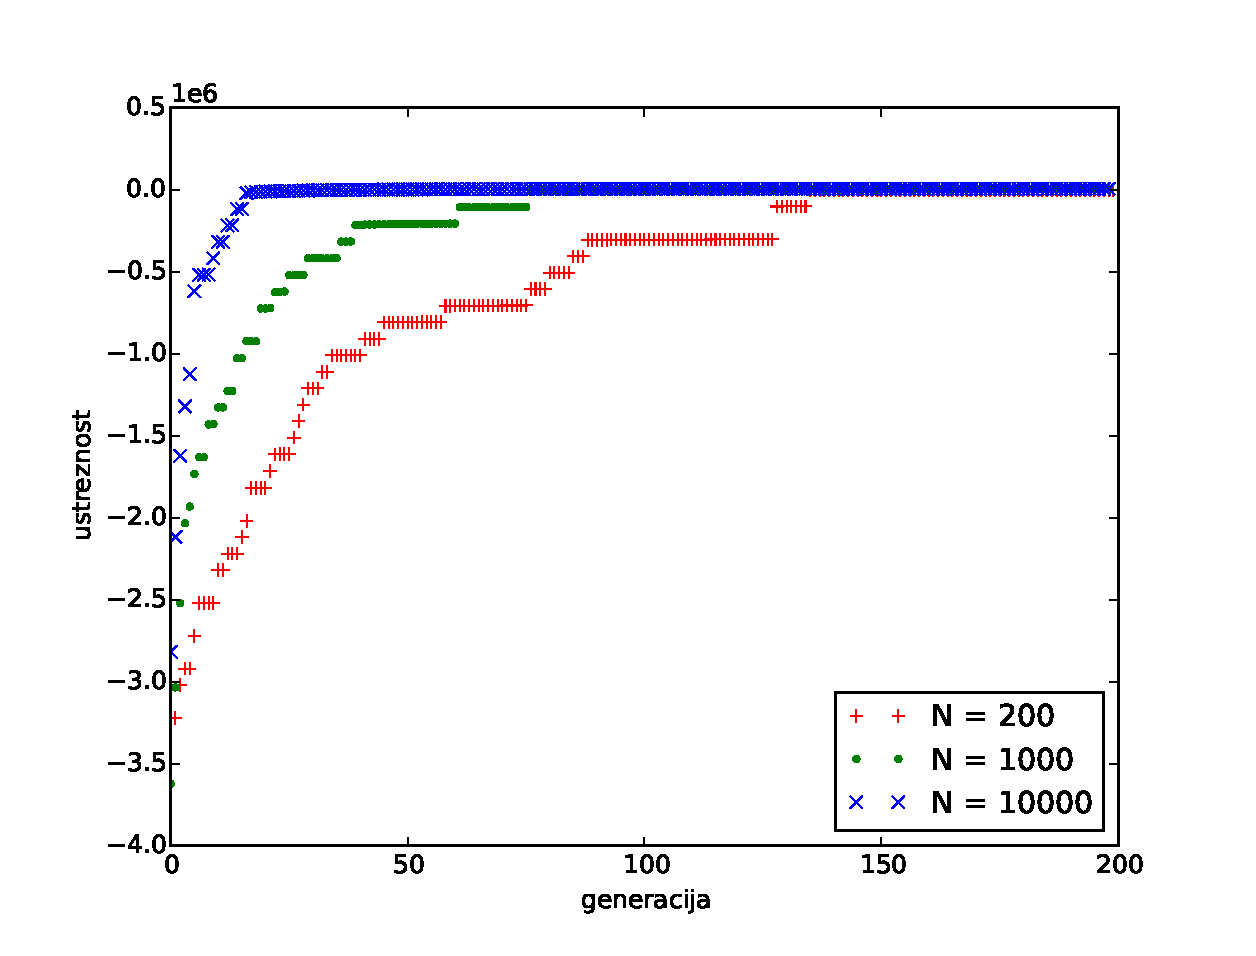
\includegraphics[scale=0.6]{res/generation-fitness-multiple.eps}
	\caption{Konvergenca vrednosti kriterijske funkcije rešitve za tri velikosti populacije. }
	\label{pic:generation-fitness-multiple}
\end{figure}

\section{Generiranje realnega urnika}
Poskusili smo tudi generirati urnik z realnimi podatki, da bi ugotovili, ali je naša implementacija primerna in uporabna tudi za realne probleme. Uporabili smo podatke Fakultete za računalništvo informatiko Univerze v Ljubljani za poletni semester študijskega leta 2014/15. Podatki zavzemajo 25 učilnic, 110 profesorjev in asistentov, 64 predmetov ter 1498 študentov. Velika razlika med temi podatki ter testnim naborom je ta, da so tukaj študenti izjemno raznoliki: nekateri imajo samo en predmet, nekateri jih imajo več kot 5. Predvsem pa je tu veliko več prekrivanj zaradi realne izbirnosti. 

Ker je podatkov v tem primeru veliko več, kot v našem testnem naboru, smo morali zmanjšati velikost populacije na 2000. Drugi parametri so ostali isti. Ustavitveni pogoj smo nastavili na 1000 generacij. Program smo poganjali na sistemih \ref{computer:virtual}, \ref{computer:old} in \ref{computer:laptop}, povezanih preko omrežja Ethernet. 

\begin{figure}
	\centering
	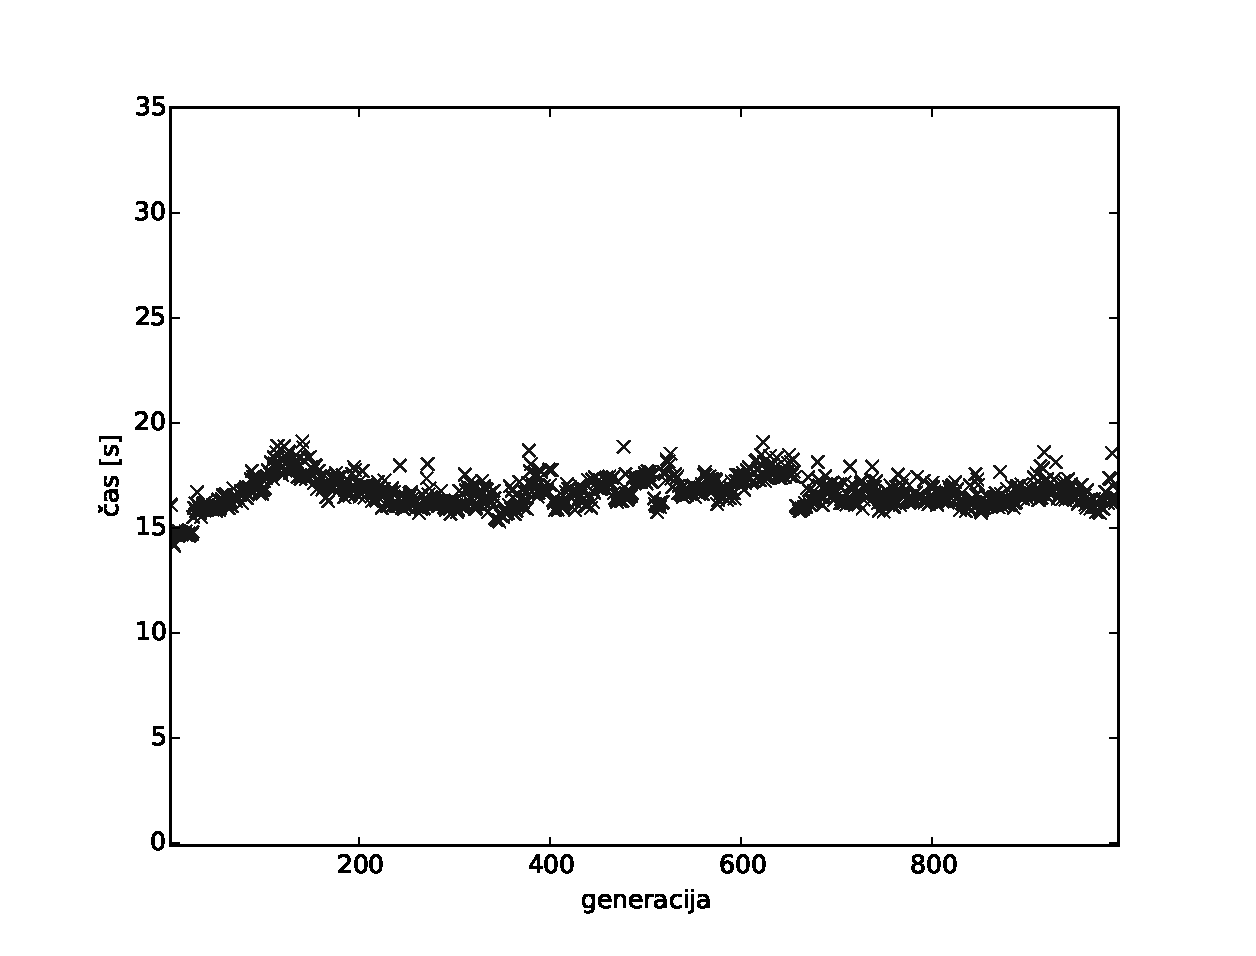
\includegraphics[scale=0.6]{res/generation-time-three-eth-REAL.eps}
	\caption{Časi, potrebni za vsako generacijo realnih podatkov. }
	\label{pic:generation-time-REAL}
\end{figure}

Skupen čas izvajanja programa je bil $4{,}6$ ur, povprečen čas za izračun ene generacije pa $16{,}7$ sekunde. Slika \ref{pic:generation-time-REAL} kaže zelo konstanten čas izvajanja programa skozi generacije. Podobno kot pri testnem naboru je program tekel 82 \% časa paralelno, 18 \% časa je porabil za komunikacijo, poraba pomnilnika vsakega od 12 procesov pa se je gibala okoli 600 MB. Končna vrednost kriterijske funkcije je bila $-274833$, kar je zavzemalo 544 (od začetnih 3514) pojavitev prekrivanj študentom. 

\begin{figure}
	\centering
	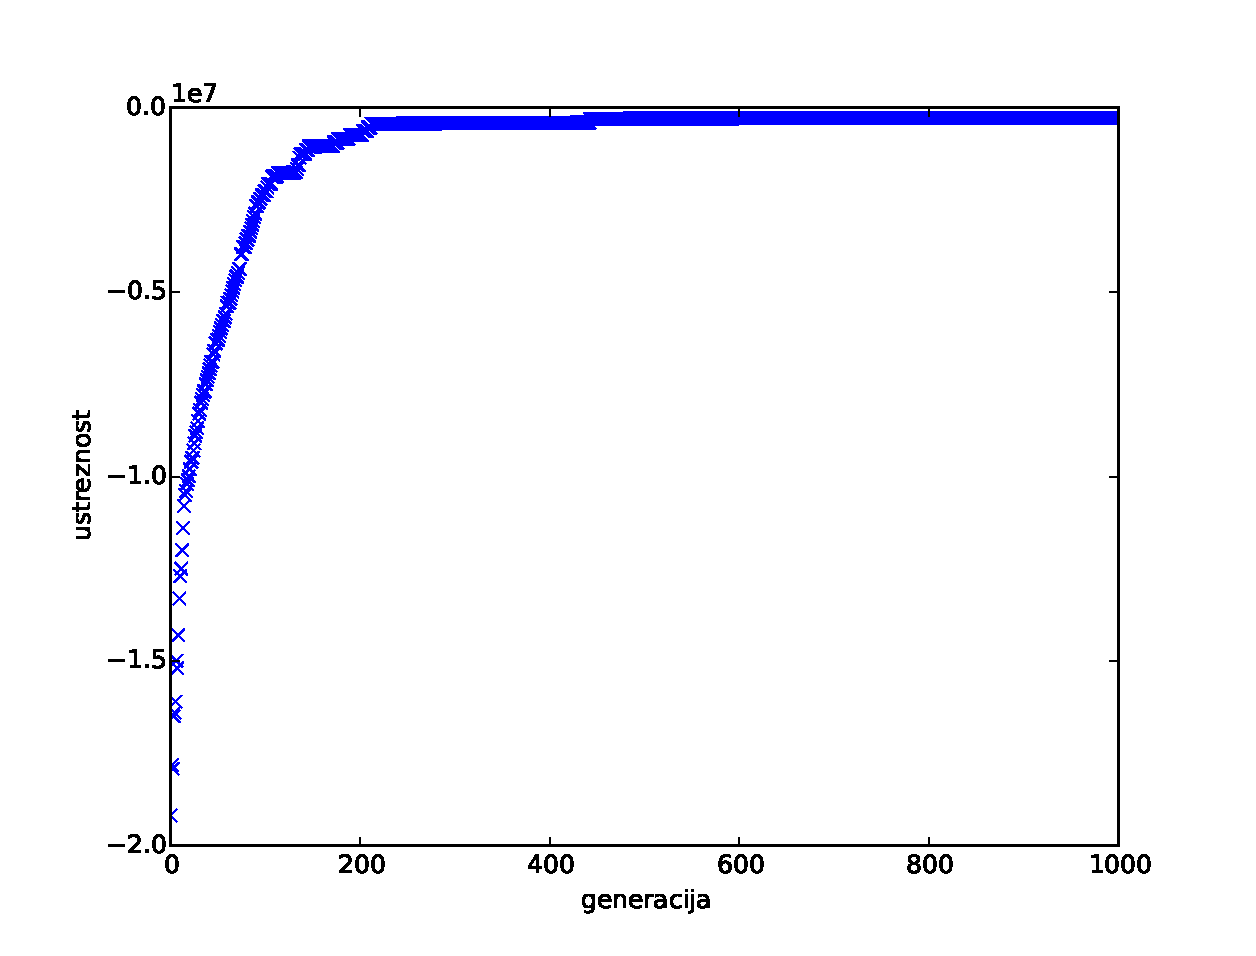
\includegraphics[scale=0.5]{res/generation-fitness-REAL.eps}
	\caption{Vrednosti kriterijske funkcije skozi generacije realnih podatkov. }
	\label{pic:generation-fitness-REAL}
\end{figure}

\begin{figure}
	\centering
	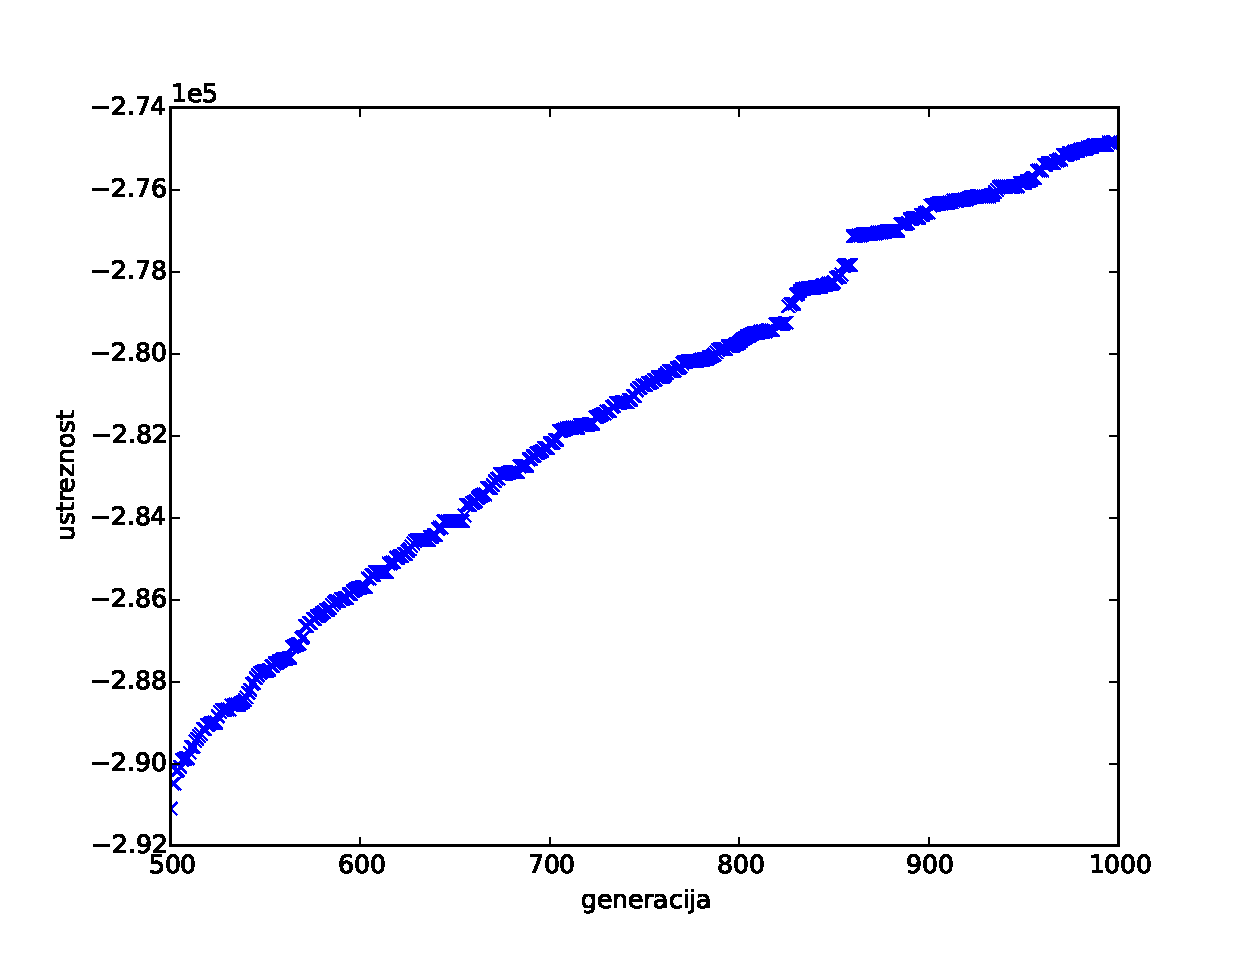
\includegraphics[scale=0.5]{res/generation-fitness-REAL-500up.eps}
	\caption{Vrednosti kriterijske funkcije za generacije nad 500 v realnih podatkih. }
	\label{pic:generation-fitness-REAL-500up}
\end{figure}

Slika \ref{pic:generation-fitness-REAL} prikazuje hitro naraščanje vrednosti kriterijske funkcije na začet\-ku, nato pa ustalitev. Če pogledamo samo generacije od polovice naprej (slika \ref{pic:generation-fitness-REAL-500up}) opazimo, da se vrednosti še vedno stalno dvigujejo, a izjemno počasi. Ta problem je mnogo večji od našega testnega nabora. Zaradi veliko večjega problemskega prostora, predvsem zaradi veliko dodatnih študentov z nenavadnimi vzorci predmetov, je težko najti optimalno rešitev. 

Sklepamo, da naš način reševanja problema ni najbolj primeren za probleme tega velikostnega reda. Za boljše rezultate bi morali implementirati lokalno iskanje, podobno kot v \cite{abdullah2008generating}, ali pa nekakšno funkcijo delnega popravljanja urnika, da bi, na primer, pametno prerazporedili študente, namesto da se popolnoma zanašamo na naključnost. Večji uspeh bi morda lahko tudi dosegli z združevanjem ekvivalentnih študentov v skupine tako, da bi imeli vsi študenti v isti skupini iste predmete. 

Kljub vsemu pa smo ugotovili, da algoritem in paralelizacija programa vzdržita tudi večje in bolj kompleksne nabore podatkov, saj se časi niso povečali eksponentno, prav tako pa je bila obvladljiva poraba pomnilnika. 

\chapter{Zaključek in nadaljnje delo}
V delu smo obravnavali popularne metode generiranja urnikov. Najprej smo preučili obstoječe pristope in pretehtali njihove prednosti ter slabosti, nato pa izbrali ustreznega, ki se sklada z našimi željami. Veliko pozornosti smo posvetili predstavitvi podatkov, saj smo s pametno shemo prihranili prostor in si olajšali implementacijo operatorjev evolucijskega algoritma. Izbrali smo tudi ustrezno paralelizacijsko ogrodje, ki se sklada z značilnostmi izvajanja programa. 

Ustvarili smo več XML shem, s katerimi smo omogočili validacijo vhodnih podatkov še pred zagonom programa. Implementirali smo evolucijski algoritem in vanj vključili netrivialne omejitve. Za hiter izračun smo uporabili namenske podatkovne strukture in tako dosegli obvladljivo časovno kompleksnost. Uspešno smo izvedli tudi paralelizacijo, saj smo dosegli dobro skalabilnost in obvladljivost pri različnih velikostih problema. Predstavitev rezultata smo realizirali s spletno aplikacijo, ki sprejme izvožen urnik in ga prikaže na uporabniku prijazen način. 

Rezultati na generiranih podatkih so bili vzpodbudni. Problem smo lahko učinkovito in kvalitetno rešili v zglednem času. Pohitritve z večjim številom jeder so bile dobre. Analizirali smo vpliv manj stabilnega omrežja z večjo latenco na čase generiranja generacij ter pregledali porabo pomnilnika na različnih velikostih problema ter različnim številom procesov. Ugotovili smo, da se poraba pomnilnika v obeh primerih veča linearno, kar je odličen rezultat. Generirati smo poskusili tudi urnik z realnimi podatki. Program na tako velikem problemu ni deloval najbolje, saj je prepočasi konvergiral k rešitvi. Predlagali smo rešitve in izboljšave, ki bi pripomogle k izboljšanju programa za večje in bolj kompleksne probleme. 

V nadaljnjem delu se je v prvi vrsti potrebno osredotočiti na predloge izboljšav algoritma, saj je pomembno, da je program uporaben tudi za večje probleme. Možne nadgradnje so analiza kompresije pošiljanja --- s tem bi lahko zmanjšali čas, ki ga program porabi za komunikacijo, delitev na lokalne in globalne izračune, kjer bi si procesi na istem sistemu vedno izmenjevali preživele, vsakih $n$ generacij pa bi se preživeli preposlali tudi preko sistemov. Lahko bi dodali tudi dodatne omejitve iz realne domene, ki temeljijo na specifičnih željah izvajalcev ali študentov. Uporabna nadgradnja bi bila inkrementalno popravljanje urnika: če bi spremenili termin enemu vnosu, bi se urnik samodejno prilagodil spremembi. Prav tako bi bile uporabne izboljšave uporabniške izkušnje, kot je grafični vmesnik za poganjanje programa ter spremljanje napredka v realnem času. 


\bibliographystyle{IEEEtran}
\bibliography{literature}


\end{document}
